%----------------------------------------------------------------
%
%  File    :  thesis.tex
%
%  Author  :  Keith Andrews, ISDS, TU Graz, Austria
%
%  Created :  30 Jul 1997
% 
%  Changed :  22 Jan 2021
%
%----------------------------------------------------------------

\documentclass[11pt]{book}

\usepackage[
a4paper,
twoside,
top=5mm,                % top margin
bottom=7mm,             % bottom margin
inner=20mm,             % inner margin (next to binding)
outer=20mm,             % outer margin (opposite binding)
bindingoffset=10mm,     % on binding side
includeheadfoot,        % include head(er) and foot(er)
headheight=10mm,        % height of header
headsep=15mm,           % sep between header and text body
footskip=15mm,          % sep between body and baseline of footer
footnotesep = 10mm plus 2mm minus 0mm  % bottom of body to top of footnote
]{geometry}
% A4 paper is w=210m, h=297mm


\newcommand{\thisdate}{10 Nov 2021}  % date of this version
\newcommand{\thisyear}{2021}         % year of this version


\newcommand{\fullh}{24cm}         % height of figures for 1 per page
\newcommand{\halfh}{9.5cm}        % height of figures for 2 per page
\newcommand{\thirdh}{6cm}         % height of figures for 3 per page


\setlength{\parindent}{1em}       % less indentation
\setlength{\parskip}{1.5ex plus 0.3ex minus 0.3ex}  % vert. space before para


% \tolerance is set by LaTeX to 200
% \sloppy sets \tolerance = 9999
% which allows LaTeX more tolerance in adding word spacing

% \sloppy
% \fussy
% \tolerance = 1000

\tolerance=400 
% makes some lines with lots of white space, but      
% tends to prevent words from sticking out in the margin



\setcounter{secnumdepth}{3}     % lowest section level still numbered
\setcounter{tocdepth}{2}        % lowest section level entered in ToC

\usepackage[T1]{fontenc}        % 8-bit output chars (must be before inputenx)
\usepackage[utf8]{inputenx}     % input char encoding

\usepackage[english,austrian,british]{babel}

\usepackage{newtxtext}          % newer times fonts
\usepackage{newtxmath}

\usepackage{relsize}            % relative font sizes \smaller \larger
\usepackage{float}              % H for float placement
\usepackage{setspace}           % adjust line spacing

\usepackage{textcomp}           % symbols such as \texttimes and \texteuro
\usepackage{latexsym}
\usepackage{fontawesome}        % fontawesome symbols

\usepackage{siunitx}            % prettier number formatting
\sisetup{%
	group-separator={,},
	group-minimum-digits=4,
}
\usepackage[super]{nth}         % 1st, 2nd, 3rd, etc.

\usepackage{xspace}
\usepackage{xstring}            % string manipulation macros
\usepackage{xparse}             % commands with optional arguments
\usepackage{etoolbox}           % for \newrobustcmd
\usepackage{makecmds}           % for \makecommand
\usepackage{calc}               % for math calculations


\usepackage[svgnames,table,xcdraw]{xcolor}
\definecolor{darkgreen}{rgb}{0.0,0.2,0.0}
\definecolor{darkblue}{rgb}{0.0,0.0,0.2}
\definecolor{darkred}{rgb}{0.2,0.0,0.0}
\definecolor{verylightgrey}{gray}{0.95}
\definecolor{lightgrey}{gray}{0.9}
\definecolor{grey}{gray}{0.7}
\definecolor{black}{gray}{0.0}

\definecolor{tableheadercolour}{gray}{0.8}
\definecolor{tablerowcolour}{gray}{0.93}

\usepackage{longtable}
\usepackage{multirow}
\usepackage{tabularx}

% Define some new column types for tables:
% like X but flushleft (= raggedright) rather than justified
\newcolumntype{Y}{>{\raggedright\arraybackslash}X}
% a p column but flushleft (= raggedright) rather than justified
\newcolumntype{L}[1]{>{\raggedright\arraybackslash}p{#1}}
% a p column but flushright (= raggedleft) rather than justified
\newcolumntype{R}[1]{>{\raggedleft\arraybackslash}p{#1}}


\usepackage{booktabs}           % nicer tables

\newcommand{\tablestretch}
{\renewcommand{\arraystretch}{1.20}}  % spacing between table rows




\usepackage{verbdef}            % define robust verb strings
\usepackage{verbatim}
\usepackage{comment}



% better lists
\usepackage{enumitem}

\setlist{
	topsep=0pt,
	partopsep=0pt,
	parsep=0.6ex,
	itemsep=1.2ex,
	left=\parindent .. 2\parindent,    % bullet .. start ot text
}

\setlist[description]{
	style=sameline,
}

% acronyms
\usepackage[nolist,nohyperlinks]{acronym}
\begin{acronym}
	\acro{vpn}[VPN]{Virtual Private Network}
	\acro{ipsec}[IPsec]{Internet Protocol Security}
	\acro{ike}[IKE]{Internet Key Exchange protocol}
	\acro{sul}[SUL]{system under learning}
	\acro{sut}[SUT]{system under test}
	\acro{pal}[PAL]{passive automata learning}
	\acro{aal}[AAL]{active automata learning}
	\acro{mat}[MAT]{minimally adequate teacher}
	\acro{ah}[AH]{Authentication Header}
	\acro{esp}[ESP]{Encapsulating Security Payload}
	\acro{isakmp}[ISAKMP]{Internet Security Association and Key Management Protocol}
	\acro{sa}[SA]{Security Association}
	\acro{vm}[VM]{virtual machine}
	\acro{afl}[AFL]{american fuzzy lop}
	\acro{dfa}[DFA]{deterministic finite automata}
	\acro{mid}[M-ID]{message-ID}
	\acro{iv}[IV]{initialization vector}
\end{acronym}


% use caption and subfig (caption2 and subfigure are now obsolete)

\usepackage[
position=bottom,
margin=1cm,
font=small,
labelfont={bf,sf},
format=plain,
indention=5mm,
aboveskip=4mm,
belowskip=0mm,
]{caption,subfig}

\captionsetup[subfigure]{
	margin=0pt,
	parskip=0pt,
	indention=5mm,
	farskip=4mm,            % skip above subfig (assuming captions at bottom)
	captionskip=2mm,        % skip between subfig and subcaption
}



\usepackage{listings}                 % for listings of source code

\makeatletter
\newlength{\numwidth}%
\setlength{\numwidth}{\widthof{\normalfont{\lst@numberstyle{99}}}}% Up to 2-digit (99) line numbers
\def\lst@PlaceNumber{%
	\makebox[\numwidth+1em][l]{%
		\makebox[\numwidth][r]{\normalfont\lst@numberstyle{\thelstnumber}}%
	}%
}
\makeatother

% lstset strategy: define defaults here for
% all non-floating (displayed) listings
% floated listings override these settings later

\lstset{                              % set parameters for listings
	floatplacement=tp,                  % default float placement
	numberbychapter,
	inputencoding=utf8,
	language=,                          % empty = plain text
	tabsize=2,
	xleftmargin=2\parindent,
	xrightmargin=2\parindent,
	frame=none,
	framexleftmargin=0mm,
	rulesepcolor=\color{verylightgrey},
	numbers=left,
	stepnumber=1,
	numberstyle=\scriptsize,
	numbersep=2ex,
	breaklines,
	showtabs=false,
	showspaces=false,
	showstringspaces=false,
	%
	basicstyle=\small\ttfamily,
	keywordstyle=\color{black},
	identifierstyle=\color{black},
	commentstyle=\color{SteelBlue},
	stringstyle=\color{black},
	%
	captionpos=b,
	abovecaptionskip=\abovecaptionskip,
	belowcaptionskip=\belowcaptionskip,
	extendedchars=true,           % listings usually only support 7-bit ascii chars
	literate=%                    % map some one-byte utf8 chars for use in listings
	%    { }{{~}}1                   % non-breaking space
	{©}{{\textcopyright}}1
	{€}{{\texteuro}}1
	{Ö}{{\"O}}1
	{Ä}{{\"A}}1
	{Ü}{{\"U}}1
	{ß}{{\ss}}1
	{ö}{{\"o}}1
	{ä}{{\"a}}1
	{ü}{{\"u}}1,
}


\lstdefinelanguage{biblatex}   % based on biblatex v 2.7a from 2013-07-14
{
	keywords={%
		@article,@book,@mvbook,@inbook,@bookinbook,@suppbook,%
		@booklet,@collection,@mvcollection,@incollection,@suppcollection,%
		@manual,@misc,@online,@patent,@periodical,@suppperiodical,%
		@proceedings,@mvproceedings,@inproceedings,@reference,@mvreference,%
		@inreference,@report,@set,@thesis,@unpublished,@xdata,%
		@conference,@electronic,@mastersthesis,@phdthesis,@techreport,@www,%
		@artwork,@audio,@bibnote,@commentary,@image,@jurisdiction,@legislation,%
		@legal,@letter,@movie,@music,@performance,@review,@software,%
		@standard,@video%
	},
	sensitive=false,
	comment=[l][\itshape]{@comment},
	morecomment=[l]{\%},
}

\lstdefinelanguage{CSS}
{
	alsoletter={-},
	morekeywords={%
		color,background,background-color,margin,padding,font,
		font-family,weight,%
		display,position,top,left,right,bottom,list,%
		style,border,size,white,space,min,width%
	},
	sensitive=false,
	morecomment=[l]{//},
	morecomment=[s]{/*}{*/},
	morestring=[b]",
}

% very simple highlighting for listings
% only highlight comments and strings

\lstdefinelanguage{SVG}
{
	morestring=[b]",
	morecomment=[s]{<!--}{-->},
	commentstyle=\color{DarkOliveGreen},
	stringstyle=\color{Navy},
	identifierstyle=\color{black},
	keywordstyle=\color{black},
}


\lstdefinelanguage{TypeScript}
{
	keywords= {break, case, catch, continue, debugger, default, delete, do, else,
		finally, for, function, if, in, instanceof, new, return, switch,
		this, throw, try, typeof, var, void, while, with, await, async,
		case, catch, class, const, default, do, enum, export, extends,
		finally, from, implements, import, instanceof, let, static, super,
		switch, throw, try},
	morecomment=[l]{//},
	morecomment=[s]{/*}{*/},
	morestring=[b]',
	morestring=[b]",
	morestring=[b]`, % Interpolation strings.
	sensitive=true,
	commentstyle=\color{DarkOliveGreen},
	stringstyle=\color{Navy},
	identifierstyle=\color{black},
	keywordstyle=\color{black},
}






\usepackage[compact,nobottomtitles,pagestyles,explicit]{titlesec}
% when using explicit, must explicitly include #1 for titlename

% nobottomtitles
% move section headings close to page bottom to next page
\renewcommand{\bottomtitlespace}{2cm}

% \chaptermark sets the value of \chaptertitle for later
% \@chapapp is defined as \chaptername outside the appendix,
% and as \appendixname within the appendix.
\makeatletter
\titleformat{\chapter}
[display]                                            % shape
{\chaptermark{\thechapter~~#1}\sffamily\bfseries}    % format
{\huge\@chapapp\ \thechapter}                        % label
{4ex}                                                % sep
{\Huge#1}                                            % before-code
\makeatother

\titleformat{name=\chapter,numberless}
[block]                                              % shape
{\chaptermark{#1}\sffamily\bfseries}                 % format
{}                                                   % label
{0ex}                                                % sep
{\Huge#1}                                            % before-code

\titleformat{\section}
{\normalfont\Large\sffamily\bfseries}{\thesection}{0.8em}{#1}

\titleformat{\subsection}
{\normalfont\large\sffamily\bfseries}{\thesubsection}{0.8em}{#1}

\titleformat{\subsubsection}
{\normalfont\normalsize\sffamily\bfseries}{\thesubsubsection}{0.8em}{#1}

\titleformat{\paragraph}[runin]
{\normalfont\normalsize\sffamily\bfseries}{\theparagraph}{0.8em}{#1}

\titleformat{\subparagraph}[runin]
{\normalfont\normalsize\sffamily\bfseries}{\thesubparagraph}{0.8em}{#1}


% vertical spacing before and after section titles
\titlespacing*{\section}
{0pt}{3.5ex plus 0.5ex minus 0.5ex}{0ex plus 0ex minus 0.2ex}

\titlespacing*{\subsection}
{0pt}{2.5ex plus 0.5ex minus 0.5ex}{0ex plus 0ex minus 0.2ex}

\titlespacing*{\subsubsection}
{0pt}{2ex plus 0.5ex minus 0.5ex}{0ex plus 0ex minus 0.2ex}

\titlespacing*{\paragraph}
{0pt}{1.5ex plus 0.3ex minus 0.3ex}{0ex plus 0ex minus 0.15ex}

\titlespacing*{\subparagraph}
{0pt}{1ex plus 0.2ex minus 0.2ex}{0ex plus 0ex minus 0.1ex}


% define page headings how I want them

\newpagestyle{main}[\small]{
	% \addtolength\headheight{6.7pt}
	% \headrule
	\sethead%
	[{\parbox[t]{0.3\textwidth}%                    % even left
		{\sffamily\thepage}}]
	[]%                                             % even centre
	[{\parbox[t]{0.6\textwidth}%                    % even right
		{\raggedleft\sffamily\chaptertitle}}]
	{{\parbox[t]{0.6\textwidth}%                    % odd left
			{\sffamily\sectiontitle}}}%
	{}%                                             % odd centre
	{{\parbox[t]{0.3\textwidth}%                    % odd right
			{\raggedleft\sffamily\thepage}}}
}





\usepackage{titletoc}

% \contentsmargin{2.55em}

\titlecontents{chapter}%
[1.5em]%                         % left indent to entry text
{\addvspace{1em}\bfseries}%      % above-code per entry
{\contentslabel{1.5em}}%         % format for numbered entry
{\hspace*{-1.5em}}%              % format for unnumbered entry
{\hfill\contentspage}%           % [no dots] and page num per entry


% Note: \dottedcontents is short form of \titlecontents

\dottedcontents{section}%
[3.8em]%                         % left indent to entry text = 1.5 + 2.3
{}%                              % above-code per entry
{2.3em}%                         % label width
{1pc}%                           % space around the dots

\dottedcontents{subsection}%
[7.4em]%                         % left indent to entry text = 3.8 + 3.6
{}%                              % above-code per entry
{3.6em}%                         % label width
{1pc}%                           % space around the dots


\dottedcontents{figure}%         % LoF entries
[3.0em]%                         % left indent to entry text = 3.8 + 3.6
{}%                              % above-code per entry
{3.0em}%                         % label width
{1pc}%                           % space around the dots

\dottedcontents{table}%          % LoT entries
[3.0em]%                         % left indent to entry text = 3.8 + 3.6
{}%                              % above-code per entry
{3.0em}%                         % label width
{1pc}%                           % space around the dots



% List of Listings is unknown to titletoc, define here

% Add extra per-chapter space to LoL to mimic LoF and LoT
% (requires package etoolbox)
\makeatletter
\patchcmd{\@chapter}% <cmd>
{\addtocontents}% <search>
{\addtocontents{lol}{\protect\addvspace{10\p@}}% add per-chapter space
	\addtocontents}% <replace>
{}{}% <success><failure>
\makeatother

% Configure LoL to mimic LoF and LoT
\contentsuse{lstlisting}{lol}

\titlecontents{lstlisting}%
[3.0em]%                              % left indent
{\addvspace{1.5mm}}%                  % above-code per entry
{\contentslabel{3.0em}}%              % format for numbered entry
{\hspace*{-3.0em}}%                   % format for unnumbered entry
{\titlerule*[1pc]{.} \contentspage}%  % dots and page num per entry
[]%                                   % below-code per entry

\renewcommand{\lstlistlistingname}{List of Listings}






% sensible settings for floats

\setlength{\textfloatsep}{9mm plus 2mm minus 2mm}
\setlength{\floatsep}{9mm plus 2mm minus 2mm}
\setlength{\intextsep}{9mm plus 2mm minus 2mm}

\setlength{\dbltextfloatsep}{9mm plus 2mm minus 2mm}
\setlength{\dblfloatsep}{9mm plus 2mm minus 2mm}

\setlength{\abovecaptionskip}{4mm plus 2mm minus 1mm}
\setlength{\belowcaptionskip}{2mm plus 1mm minus 1mm}

% See http://www-rohan.sdsu.edu/~aty/bibliog/latex/floats.html
% See https://robjhyndman.com/hyndsight/latex-floats/

\setcounter{topnumber}{2}               % max num floats at top of page
\setcounter{dbltopnumber}{2}            % max num floats on 2col page
\setcounter{bottomnumber}{2}            % max num floats at bottom of page
\setcounter{totalnumber}{4}             % max num floats on a page

\renewcommand{\topfraction}{0.8}        % max fraction of floats at top
\renewcommand{\dbltopfraction}{0.9}     % max fraction of floats at top 2col
\renewcommand{\bottomfraction}{0.8}     % max fraction of floats at bottom
\renewcommand{\textfraction}{0.2}       % min fraction of text

% only for entirely float pages:
\renewcommand{\floatpagefraction}{0.7}      % min page fraction having floats
\renewcommand{\dblfloatpagefraction}{0.7}   % min 2col page fraction having floats


\usepackage[section,above,below]{placeins}  % keep floats to their own section





\usepackage[short]{datetime}   % load datetime *after* babel, requires fmtcount
% \newdateformat{britdate}{%
	% \ordinaldate{\THEDAY} \,\monthname[\THEMONTH] \THEYEAR
	% }
\newdateformat{unixdate}{%
	\twodigit{\THEDAY}~\shortmonthname[\THEMONTH]~\THEYEAR
}

% TODO: use new datetime2 instead of datetime



\usepackage[
autostyle=true,          % adapt quote style to current language
english=british,         % british english as default
threshold=1,             % set block quotations >1 line in display mode
maxlevel=4,              % max nesting level
]{csquotes}

\usepackage[
indentfirst=false,
vskip=0pt,               % by default would be \topsep + \partopsep.
]{quoting}

% tell csquotes to use quoting environment
% for \displayquote and \blockquote
\SetBlockEnvironment{quoting}

% if cite is issued by a csquote command
\renewcommand{\mkcitation}[1]{\space#1}

% I prefer double quotes as outer
\DeclareQuoteStyle{keithbritish}%  [variant]{style}
{\textquotedblleft}%                      opening outer mark
{\textquotedblright}%                     closing outer mark
[0.05em]%
{\textquoteleft}%                         opening inner mark
{\textquoteright}%                        closing inner mark

\ExecuteQuoteOptions{style=keithbritish}





\usepackage[
backend=biber,
%  style=ext-authoryear-comp,   % defined in biblatex-ext package
style=ext-authoryear,        % defined in biblatex-ext package
sorting=nyt,
useprefix,                   % van and von are part of second name
mergedate=false,             % only for authoryear style
dashed=false,                % only for authoryear style
abbreviate=false,
maxcitenames=2,              % if > 2 authors,
mincitenames=1,              % use first 1 then et al
maxbibnames=99,              % if > 99 authors,
minbibnames=6,               % use first 6 then et al
uniquelist=minyear,
uniquename=init,
hyperref=true,
backref=true,
backrefstyle=two,
sortlocale=en,
]{biblatex}


% set for csquotes, but \autocite only available
% after biblatex is loaded
\SetCiteCommand{\autocite}    % or maybe \parencite

% more space between entries in bib
\setlength\bibitemsep{1.5\itemsep}

% kandrews: replace round brackets with square brackets in citations
\DeclareOuterCiteDelims{parencite}{\bibopenbracket}{\bibclosebracket}
\DeclareInnerCiteDelims{textcite}{\bibopenbracket}{\bibclosebracket}

% kandrews: replace round brackets with square brackets in bibliography
% biblabeldate is a biblatex-ext feature
\DeclareFieldFormat{biblabeldate}{\mkbibbrackets{#1}}


% remove URL: from in front of URLs
\DeclareFieldFormat{url}{\url{#1}}
\DeclareFieldFormat{doi}{\doi{#1}}
\DeclareFieldFormat{isbn}{\isbn{#1}}
\DeclareFieldFormat{issn}{\issn{#1}}

% suppress urldate field
\AtEveryBibitem{\clearfield{urlyear}}

% remove In: from aricles and inproceedings entries
% https://tex.stackexchange.com/questions/10682/suppress-in-biblatex
\renewbibmacro{in:}{%
	\ifboolexpr{%
		test {\ifentrytype{article}}%
		or
		test {\ifentrytype{inproceedings}}%
	}{}{\printtext{\bibstring{in}\intitlepunct}}%
}

% make all entry titles italic
% (also removes quotation marks from around titles)
% https://tex.stackexchange.com/questions/311816/want-title-in-simple-numeric-not-italic-through-bibliography
\DeclareFieldFormat*{title}{\mkbibitalic{#1}}
\DeclareFieldFormat*{citetitle}{\mkbibitalic{#1}}

% make journal names non-italic
\DeclareFieldFormat{journaltitle}{#1\isdot}

% make proceedings names non-italic
\DeclareFieldFormat[inproceedings]{booktitle}{#1\isdot}

% use nth for edition
\DeclareFieldFormat{edition}{%
	\ifinteger{#1}
	{\nth{#1}~\bibstring{edition}}
	{#1\isdot}}

% overwrite some standard strings in english.lbx
\DefineBibliographyStrings{english}{%
	edition          = {Edition},
	mathesis         = {Master's Thesis},
	phdthesis        = {PhD\addabbrvspace Thesis},
}


% kandrews
% use Unix format for dates in biblio:
% 29 Dec 2015, 01 Oct 2018, etc.

% for now, define under lang english not british
% due to bug in biblatex 3.11

\DefineBibliographyStrings{english}{%
	january          = {Jan},
	february         = {Feb},
	march            = {Mar},
	april            = {Apr},
	may              = {May},
	june             = {Jun},
	july             = {Jul},
	august           = {Aug},
	september        = {Sep},
	october          = {Oct},
	november         = {Nov},
	december         = {Dec},
}

\DefineBibliographyExtras{english}{%
	% #1 = year, #2 = month, #3 = day
	\protected\def\mkbibdatelong#1#2#3{%
		\iffieldundef{#3}
		{}
		{\mkdayzeros{\thefield{#3}}%
			\iffieldundef{#2}{}{\nobreakspace}}%
		\iffieldundef{#2}
		{}
		{\mkbibmonth{\thefield{#2}}%
			\iffieldundef{#1}{}{\space}}%
		\iffieldbibstring{#1}{\bibstring{\thefield{#1}}}{\mkyearzeros{\thefield{#1}}}}%
	%
	\protected\def\mkbibdateshort#1#2#3{%
		\iffieldundef{#3}
		{}
		{\mkdayzeros{\thefield{#3}}%
			\iffieldundef{#2}{}{\nobreakspace}}%
		\iffieldundef{#2}
		{}
		{\mkbibmonth{\thefield{#2}}%
			\iffieldundef{#1}{}{\space}}%
		\iffieldbibstring{#1}{\bibstring{\thefield{#1}}}{\mkyearzeros{\thefield{#1}}}}%
}



\addbibresource{bibliography.bib}
\addbibresource{writing.bib}



% xurl provides better URL breaking than url
% load after biblatex
\usepackage[hyphens,obeyspaces]{xurl}
\def\UrlFont{\smaller\ttfamily}





% adapt pdftitle, pdfsubject, pdfauthor, pdfkeywords
% for your survey paper

\usepackage{ifpdf}

\ifpdf
% pdflatex
\usepackage[pdftex]{graphicx}
\DeclareGraphicsExtensions{.pdf,.jpg,.png}
\pdfcompresslevel=9
\pdfobjcompresslevel=1  % also compress PDF object streams except embedded PDFs
\pdfpageheight=297mm
\pdfpagewidth=210mm
\usepackage[            % hyperref should be last package loaded
unicode,
pdftex,
pdfversion=1.7,
pdftitle={Guidelines for Writing a Master's Thesis},
pdfsubject={Master's Thesis Template},
pdfauthor={Keith Andrews},
pdfkeywords={master's thesis, skeleton, guidelines, template},
bookmarks,
bookmarksnumbered,
linktocpage,
colorlinks,
linkcolor=darkred,
anchorcolor=red,
citecolor=darkgreen,
urlcolor=darkblue,
pdfstartview=Fit,              % initial view
pdfview=Fit,                   % view after following a link
pdfpagelayout=SinglePage,      % single page, no scrolling
pdfpagemode=UseOutlines,       % open bookmarks in Acrobat
plainpages=false,              % avoids duplicate page number problem
pdfpagelabels,                 % avoids duplicate page number problem
breaklinks=true,               % allow links exceeding a single line
]{hyperref}

\else
% latex
\usepackage[dvips]{graphicx}
\DeclareGraphicsExtensions{.eps}
\usepackage[dvips]{hyperref}
\fi

% export adjustbox keys to includegraphics
% must be after \usepackage{graphicx}
\usepackage[export]{adjustbox}    % valign=t, frame, ...

\usepackage{todonotes}

% macros and definitions

\newcommand\fname{\begingroup \smaller\urlstyle{tt}\Url}

\newcommand\vname{\begingroup \smaller\urlstyle{tt}\Url}


% for class names, define our own url style

\makeatletter  % protect @ names

% \url@letstyle: New URL sty to premit break at any letters.
% Based on \url@ttstyle

\def\Url@letdo{% style assignments for tt fonts or T1 encoding
\def\UrlBreaks{\do\a\do\b\do\c\do\d\do\e\do\f\do\g\do\h\do\i\do\j\do\k\do\l%
               \do\m\do\n\do\o\do\p\do\q\do\r\do\s\do\t\do\u\do\v\do\w\do\x%
               \do\y\do\z%
               \do\A\do\B\do\C\do\D\do\E\do\F\do\G\do\H\do\I\do\J\do\K\do\L%
               \do\M\do\N\do\O\do\P\do\Q\do\R\do\S\do\T\do\U\do\V\do\W\do\X%
               \do\Y\do\Z%
}%
\def\UrlBigBreaks{\do\.\do\@\do\\\do\/\do\!\do\_\do\|\do\%\do\;\do\>\do\]%
 \do\)\do\,\do\?\do\'\do\+\do\=\do\#\do\:\do@url@hyp}%
\def\UrlNoBreaks{\do\(\do\[\do\{\do\<}% (unnecessary)
\def\UrlSpecials{\do\ {\ }}%
\def\UrlOrds{\do\*\do\-\do\~}% any ordinary characters that aren't usually
\Urlmuskip = 0mu plus 1mu%
}

\def\url@letstyle{%
\@ifundefined{selectfont}{\def\UrlFont{\sf}}{\def\UrlFont{\sffamily}}\Url@letdo
}

\makeatother  % unprotect @ names


\newcommand\cname{\begingroup \smaller\urlstyle{let}\Url}


\newcommand{\imgcredit}[1]
{%
\small
[#1]
}


\newcommand{\chapquote}[2]
{%
\begin{quote}
\emph{%
``#1''%
}%
\begin{flushright}
{\scriptsize \sffamily [#2]}%
\end{flushright}
\end{quote}
}


% \urlfootnote{url}{day}{month}{year}
\newcommand{\murlfootnote}[4]{\footnote{\url{{#1}} (last visit {#4}-{#3}-{#2})}}
\newcommand{\murlfootnotebreak}[4]{\footnote{\url{{#1}}\\ \hspace*{6mm}(last visit {#4}-{#3}-{#2})}}

% change margin command
\def\changemargin#1#2{\list{}{\rightmargin#2\leftmargin#1}\item[]}
\let\endchangemargin=\endlist

% tikz stuff
\usepackage{tikz, wrapfig}
\usetikzlibrary{positioning, calc}




\begin{document}
	
	\unixdate
	
	\frontmatter
	
	\normalsize
	\pagestyle{empty}             % for title pages
	\pagenumbering{Roman}         % for pdf labels
	
	%----------------------------------------------------------------
%
%  File    :  thesis-title.tex
%
%  Author  :  Keith Andrews, ISDS, TU Graz, Austria
% 
%  Created :  22 Feb 1996
% 
%  Changed :  22 Jan 2021
% 
%----------------------------------------------------------------


% --- Main Title Page ------------------------------------------------


\vspace*{2cm}


\begin{center}
\begin{spacing}{1.1}
\Huge\sffamily\bfseries
Model Learning and Fuzzing of the IPsec-IKEv1 VPN Protocol\\
\end{spacing}

\vspace{3cm}

% \LARGE \sffamily Draft 0.9

\vspace{3cm}

{\LARGE\sffamily
Benjamin Wunderling
}
\end{center}



% --- English Title Page ------------------------------------------------


% based on:
% https://tu4u.tugraz.at/fileadmin/Studierende_und_Bedienstete/Formulare/Diplomarbeit_Vorlage.pdf



\cleardoublepage


\vspace*{-3cm}

\begin{center}

\includegraphics[height=1cm]{diagrams/tugraz-logo.pdf}

\vspace{2cm}

\begin{spacing}{1.1}
\huge\sffamily\bfseries
Model Learning and Fuzzing of the IPsec-IKEv1 VPN Protocol\\
\end{spacing}

\vspace{2cm}

{\Large\sffamily Benjamin Wunderling B.Sc.}

\vspace{2cm}

{\Large\sffamily\bfseries Master's Thesis}

\vspace{5mm}

{\small\sffamily to achieve the university degree of}

\vspace{5mm}

{\normalsize\sffamily Diplom-Ingenieur}

\vspace{5mm}

{\normalsize\sffamily
Master's Degree Programme: Computer Science
}


\vspace{1cm}

{\small\sffamily submitted to}

\vspace{5mm}

{\large\sffamily Graz University of Technology}



\vspace{1cm}

{\small\sffamily Supervisor}

\vspace{5mm}

{\normalsize\sffamily
Ao.Univ.-Prof.\ Dr.\ Keith Andrews \\
Institute of Interactive Systems and Data Science (ISDS)
}


\vspace{1cm}

{\normalsize\sffamily Graz, \thisdate}



\vfill

{\footnotesize\sffamily \copyright~Copyright \thisyear{} by Keith Andrews,
except as otherwise noted.}

{\footnotesize\sffamily This work is placed under a
Creative Commons Attribution 4.0 International
(\href{https://creativecommons.org/licenses/by/4.0/}{CC BY 4.0}) licence.}


\end{center}





% --- Pledge ----------------------------------------------------

\cleardoublepage

\vspace*{2cm}


% adapted from:
% https://tu4u.tugraz.at/fileadmin/Studierende_und_Bedienstete/Formulare/Diplomarbeit_Vorlage.pdf
% https://tu4u.tugraz.at/fileadmin/Studierende_und_Bedienstete/Forms/Diploma_thesis_template.pdf
% Email vom 2. Sept. 2015

% and

% Beschluss der Curricula-Kommission für Bachelor-,
% Master- und Diplomstudien vom 10.11.2008
% Genehmigung des Senates am 1.12.2008



\subsection*{Statutory Declaration}
\noindent
\textit{
I declare that I have authored this thesis independently, that I have
not used other than the declared sources / resources, and that I have
explicitly indicated all material which has been quoted either
literally or by content from the sources used. The document uploaded
to TUGRAZonline is identical to the present thesis.}

\vspace{1cm}


\begin{otherlanguage}{austrian}

\subsection*{Eidesstattliche Erklärung}
\noindent
\textit{
Ich erkläre an Eides statt, dass ich die vorliegende Arbeit
selbstständig verfasst, andere als die angegebenen Quellen/Hilfsmittel
nicht benutzt, und die den benutzten Quellen wörtlich und inhaltlich
entnommenen Stellen als solche kenntlich gemacht habe. Das in
TUGRAZonline hochgeladene Dokument ist mit der vorliegenden
Arbeit identisch.}

\vspace{2cm}

\noindent
\parbox[top]{4cm}{
\begin{center}
\underline{\hspace*{4cm}} \\
Date/Datum
\end{center}
}
%
\hfill
%
\parbox[top]{6cm}{
\begin{center}
\underline{\hspace*{6cm}} \\
Signature/Unterschrift
\end{center}
} 

\end{otherlanguage}




% --- English Abstract ----------------------------------------------------


\cleardoublepage

\vspace*{2cm}

\begin{center}
{\Large\sffamily\bfseries Abstract}
\end{center}

Writing a thesis is a vast, overwhelming endeavour. There are many
obstacles and false dawns along the way. This thesis takes a fresh
look at the process and addresses new ways of accomplishing this
daunting goal.

The abstract should concisely describe what the thesis is about and
what its contributions to the field are (what is new). Market your
contributions to your readership. Also make sure you mention all
relevant keywords in the abstract, since many readers read \emph{only}
the abstract and many search engines index \emph{only} title and
abstract.

This thesis explores the issues concerning the clear structuring and
the academic criteria for a thesis and presents numerous novel
insights. Special attention is paid to the use of clear and simple
English for an international audience, and advice is given as to the
use of technical aids to thesis production. Two appendices provide
specific local guidance.

          % Title Pages, Abstracts, Pledge
	
	
	\cleardoublepage
	\pagestyle{plain}             % for preliminary pages
	\pagenumbering{roman}         % for preliminary pages
	
	
	% TODO ka is this necessary?  see iaweb.tex
	% \phantomsection    % so hyperref pdf link jumps to correct page??
	
	\begin{spacing}{0.8}
		\tableofcontents
	\end{spacing}
	\addcontentsline{toc}{chapter}{Contents}
	
	\cleardoublepage
	\begin{spacing}{0.8}
		\listoffigures
	\end{spacing}
	\addcontentsline{toc}{chapter}{List of Figures}
	
	\cleardoublepage
	\begin{spacing}{0.8}
		\listoftables
	\end{spacing}
	\addcontentsline{toc}{chapter}{List of Tables}
	
	\cleardoublepage
	\begin{spacing}{0.8}
		\lstlistoflistings
	\end{spacing}
	\addcontentsline{toc}{chapter}{List of Listings}
	
	
	
	\cleardoublepage
	%----------------------------------------------------------------
%
%  File    :  thesis-acknowl.tex
%
%  Author  :  Keith Andrews, IICM, TU Graz, Austria
% 
%  Created :  22 Feb 1996
% 
%  Changed :  19 Mar 2008
% 
%----------------------------------------------------------------


\chapter*{Acknowledgements}
\addcontentsline{toc}{chapter}{Acknowledgements}


I am indebted to my colleagues at the ISDS and the Know-Center who
have provided invaluable help and feedback during the course of my
work.
%
I especially wish to thank my advisor, Keith Andrews, for his
immediate attention to my questions and endless hours of toil in
correcting draft versions of this thesis.

Special mention goes to
Christian Gütl,
Irene Isser, and
Josef Moser
for their help in translating the thesis abstract into German
and to
Bernhard Zwantschko and Didi Freismuth for ample supplies of coffee.
%
Please remember to replace this tongue-in-cheek acknowledgements
section with your own version!


Last but not least, without the support and understanding of my wife,
pleasant hours with my girlfriend, and the tolerance of my friends,
this thesis would not have been possible.

\vspace{2cm}


\begin{flushright}
Keith Andrews \\[1ex]
{\small Graz, Austria, \thisdate}
\end{flushright}

        	% Acknowledgements
	
	\cleardoublepage
	%----------------------------------------------------------------
%
%  File    :  vpn_creditss.tex
%
%  Author  :  Benjamin Wunderling, TU Graz, Austria
% 
%----------------------------------------------------------------


\chapter*{Credits}
\addcontentsline{toc}{chapter}{Credits}

I would like to thank the following individuals and organisations for
permission to use their material:
\begin{itemize}
\item The thesis was written using Keith Andrews' skeleton
  thesis \parencite{KeithThesis}.

\end{itemize}


        	% Credits
	
	
	
	\mainmatter
	
	\cleardoublepage
	\pagestyle{main}            % for main pages
	\pagenumbering{arabic}      % for main pages
	
	% Part 1 Embedding
	
	\cleardoublepage
	%----------------------------------------------------------------
%
%  File    :  thesis-embed.tex
%
%  Author  :  Benjamin Wunderling, TU Graz, Austria
% 
%----------------------------------------------------------------

\chapter{Introduction}

\label{chap:Introduction}

% Background
\section{Motivation}
\ac{vpn} are used to allow secure communication over an insecure channel. They function by creating a secure encrypted tunnel through which users can send their data. Example use cases include additional privacy from prying eyes such as Internet Server Providers, access to region-locked online content and secure remote access to company networks. The importance of \ac{vpn} software has increased dramatically since the beginning of the COVID-19 pandemic due to the influx of people working from home \cite{DBLP:journals/cacm/FeldmannGLPPDWW21}. This makes finding vulnerabilities in \ac{vpn} software more critical than ever. % state reports on damages by vpn errors? 
% IPSEC
\ac{ipsec} is a popular \ac{vpn} protocol suite and most commonly uses the \ac{ike} protocol to share authenticated keying material between involved parties. Therefore, \ac{ike} and \ac{ipsec} are sometimes used interchangeably. We will stick to the official nomenclature of using \ac{ipsec} for the full protocol and \ac{ike} for the key exchange only. \ac{ike} has two versions, \ac{ike}v1~\cite{rfc:ikev1} and \ac{ike}v2~\cite{rfc:ikev2}, with \ac{ike}v2 being the newer and recommended version, according to a report by the National Institute of Standards and Technology~\cite{nist791491}. However, despite \ac{ike}v2 supposedly replacing its predecessor, \ac{ike}v1, sometimes also called Cisco \ac{ipsec}, is still in widespread use today. This is reflected by the company AVM to this day only offering \ac{ike}v1 support for their popular FRITZ!Box routers \cite{avm2022}. Additionally, \ac{ike}v1 is also used for the L2TP/\ac{ipsec} protocol, one of the most popular \ac{vpn} protocols according to NordVPN \cite{nordvpn2021}. The widespread usage of \ac{ipsec}-\ac{ike}v1, combined with its relative age and many options makes it an interesting target for security testing.


\section{Research Problems and Goals}
% Automata Learning
Behavioral models are a useful tool in testing and verifying the correctness of complex systems. A model simulating the behavior of a system gives an abstract high-level overview of its inner workings, allowing for much easier understanding than code review. Additionally, the model can be used e.g. to automatically generate test cases, or to fingerprint / detect specific software implementations \cite{pferscher2021fingerprinting, pferscher2022fuzzing}. Despite their usefulness, the availability of accurate models may be limited for the several reasons. Firstly, the manual creation of an accurate behavioral model of a complex system can be a tedious and error-prone process. Secondly, the model must be updated every time the system is changed, i.e. functionality is added or changed in any way. Automata learning has proven itself as a useful technique for automatically generating behavioral models of various communication protocols, e.g. Bluetooth Low Energy~\cite{pferscher2021fingerprinting}, TCP~\cite{DBLP:conf/cav/Fiterau-Brostean16}, SSL~\cite{DBLP:conf/spin/Fiterau-Brostean17} or MQTT~\cite{DBLP:conf/icst/TapplerAB17}. 

\Ac{aal} is an automata learning technique in which a behavioral model is generated by actively querying a system to gain information about it. Notable examples of \ac{aal} algorithms include the $L^*$ algorithm by Angluin \cite{angluin1987learning} and the $KV$ algorithm by Kearns and Vazirani \cite{KV1994}.

\Ac{aal} is of particular interest for security testers, as it can also be applied to systems where knowledge about its inner workings is lacking, e.g. due to its implementation code being closed-source. We call such systems black-box systems. It is not unusual for \acp{vpn} and other security-critical software to be closed-source and therefore a black-box system for testers. Fortunately, \ac{aal} allows for the creation of a behavioral model of a black-box system, which can then be used for model-based testing approaches.

% Problem / motivation
By combining automata learning with fuzzing or similar software testing techniques, network protocols can be extensively and automatically tested without requiring access to their source code. Guo et al.~\cite{guo2019model} tested \ac{ipsec}-\ac{ike}v2 using automata learning and model checking, however so far, no studies have focused on \ac{ike}v1 in the context of automata learning. Therefore our goal was to black-box test the \ac{ipsec}-\ac{ike}v1 protocol using automata learning in combination with automata-based fuzzing. We used the \ac{aal} framework \textsc{AALpy} \cite{muvskardin2022aalpy} with a custom mapper to learn the state machines of various \ac{ipsec}-\ac{ike}v1 server implementations. We then further utilized the learned models for model-based fuzzing, creating a custom fuzzing framework supporting multiple types of input-sequence generation. In doing so, several deviations from the RFC specification, a potential deadlock and a cryptographic Python library bug were discovered.

% Expand this section more
\section{Structure}
This thesis is structured as follows. Chapter~\ref{chap:Related} gives an overview of the related literature. Chapter~\ref{chap:Preliminaries} introduces necessary background knowledge, covering the \ac{ipsec}-\ac{ike}v1 protocol, Mealy machines, automata learning and fuzzing. Our learning setup, custom mapper and fuzzing methodology are presented in Chapter~\ref{chap:Learning}. In Chapter~\ref{chap:Evaluation}, learned models and the results of the fuzzing tests are showcased and analyzed.
Finally, Chapter~\ref{chap:Conclusion} summarizes the thesis and discusses future work.          	% Introduction: 1-2p (split into motivation, Research Problem and Goals and Structure)
	
	\cleardoublepage
	%----------------------------------------------------------------
%
%  File    :  vpn_related.tex
%
%  Author  :  Keith Andrews, IICM, TU Graz, Austria
% 
%  Created :  22 Feb 96
% 
%  Changed :  19 Feb 2004
% 
%----------------------------------------------------------------

\chapter{Related Work}

\label{chap:Related}
% TODO: check if Feldman is correct
% TODO: add a summary of mentioned related work with each citation
The aim of this chapter is to give a brief overview of related work, focusing mainly on automata learning and testing of secure communication protocols.

Model learning is a popular tool for creating behavioral models of network and communication protocols. The learned models showcase the behavior of the \ac{sul} and can be analyzed to find differences between implementation and specification. Furthermore, the learned models can be used for additional security testing techniques, e.g., for model checking or model-based testing. 

Model learning has been applied to a variety of different protocols, including many security-critical ones. De Ruiter and Poll~\cite{DBLP:conf/uss/RuiterP15} automatically and systematically analyzed TLS implementations by using the random inputs sent during the model learning process to test the \ac{sul} for unexpected and dangerous behavior. The unexpected behavior then had to be manually examined for impact and exploitability. Tappler et al.~\cite{DBLP:conf/icst/TapplerAB17} similarly analyzed various MQTT broker/server implementations, finding several specification violations and faulty behavior. Furthermore, the 802.11 4-Way Handshake of Wi-Fi was analyzed by Stone et al.~\cite{DBLP:conf/esorics/StoneCR18} using automata learning to test implementations on various routers, finding servery vulnerabilities.
Fiterau and Brostean combined model learning with the related field of model checking, in which an abstract model is checked for specified properties to ensure correctness. In their work they learned and analyzed both TCP~\cite{DBLP:conf/cav/Fiterau-Brostean16} and SSL~\cite{DBLP:conf/spin/Fiterau-Brostean17} implementations, showcasing several implementation deviations from their respective RFC specifications.
The Bluetooth Low Energy (BLE) protocol was investigated by Pferscher and Aichernig~\cite{pferscher2021fingerprinting}. In addition to finding several behavioral differences between BLE devices, they were able to distinguish the individual devices based on the learned models, essentially allowing the identification of hardware, based on the learned model (i.e. fingerprinting).

Specifically within the domain of \acp{vpn}, Novickis et al.~\cite{novickis2016protocol} and Daniel et al.~\cite{daniel2018inferring} learned models of the OpenVPN protocol and showcased how to use the learned models to perform protocol fuzzing. In contrast to our approach, they chose to learn a more abstract model of the entire OpenVPN session, where details about the key exchange were abstracted in the learned model. 
Even more closely related to our work, Guo et al. \cite{guo2019model} used automata learning to learn and test the \ac{ipsec}-\ac{ike}v2 protocol setup to use certificate-based authentication. They used the LearnLib~\cite{software:learnlib} library for automata learning and performed model checking of the protocol, using the learned state machine. In contrast, our work focuses on the \ac{ipsec}-\ac{ike}v1 protocol, the predecessor of \ac{ipsec}-\ac{ike}v2, which has not yet been tested with methods utilizing automata learning. \Acp{psk} are used for authentication and the learned model serves as a basis for fuzz-testing. The two protocol versions differ greatly on a packet level, with \ac{ike}v1 needing more than twice the amount of packets to establish a connection than \ac{ike}v2 and also being far more complex to set up.  Guo et al. highlight the complexity of \ac{ike}v1 repeatedly in their work, which emphasizes the need to also test the older version of the protocol as well, especially seeing as it is still in widespread use today~\cite{avm2022}. Our work completes the coverage of learning-based testing approaches for both \ac{ike} versions.

\TODO{Add section on model-based fuzzing, see andrea notes for papers}			% Related work: 1 page?
	
	\cleardoublepage
	%----------------------------------------------------------------
%
%  File    :  vpn_prelim.tex
%
%  Author  :  Keith Andrews, IICM, TU Graz, Austria
% 
%  Created :  22 Feb 96
% 
%  Changed :  19 Feb 2004
% 
%----------------------------------------------------------------

\chapter{Preliminaries}

\label{chap:Preliminaries}

\iffalse
\section{Deterministic Finite Automata}
A \ac{dfa} is a finite-state machine that is defined as a quintuple $D = \{S, s_0, \Sigma, \delta, F\}$ where $S$ is a finite set of states, $s_0 \in S$ is the initial state, $\Sigma$ is a finite set called the input alphabet, $\delta$ is the state-transition function $\delta \colon S \times \Sigma \rightarrow S$ that maps a state and an element of the input alphabet to another state in $S$ and $F$ is the set of accepting states. \Acp{dfa} do not have any output.
\fi

\section{Mealy Machines}
Mealy machines are a modeling formalism for reactive systems such as communication protocols. Mealy machines are finite-state machines in which each transition is labeled with an input and a corresponding output action. More formally, a Mealy machine is defined as a 6-tuple $M = \{S, s_0, \Sigma, O, \delta, \lambda\}$, where $S$ is a finite set of states, $s_0 \in S$ is the initial state, $\Sigma$ is a finite set called the input alphabet, $O$ is a finite set called the output alphabet, $\delta$ is the state-transition function $\delta \colon S \times \Sigma \rightarrow S$ that maps a state and an element of the input alphabet to another state in $S$. In other words, the choice of each new state is defined by the current state and an external input. Finally, $\lambda$ is the output function $\lambda \colon S \times \Sigma \rightarrow O$ which maps a state-input alphabet pair to an element of the output alphabet $O$. We use Mealy machines to model the state of learned \ac{ipsec} implementations.

\section{Automata Learning}
Automata learning refers to methods of learning the state model, or automaton, of a system through an algorithm or process. Automata learning algorithms generate a model that describes the behavior of the \ac{sul}. We differentiate between active and passive automata learning. In passive automata learning, models are learned based on a given data set describing the behavior of the \ac{sul}, e.g. log files. In contrast, in \ac{aal} the \ac{sul} is queried directly. In this paper, we will focus on \ac{aal} and will, moving on, be referring to it as automata learning or \ac{aal} interchangeably. 

One of the most influential AAL algorithms was introduced in 1987 by Dana Angluin, titled ``Learning regular sets from queries and counterexamples''~\cite{ANGLUIN198787}. In this seminal paper, Angluin introduced the concept of the \ac{mat} as well as an algorithm for learning regular languages from queries and counterexamples, called $L^*$. Note, that while the $L^*$ algorithm was originally designed to learn \acp{dfa} of regular languages, it can be simply extended to work for Mealy machines by making use of the similarities between \acp{dfa} and Mealy machines~\cite{hungar2003domain, shahbaz2009inferring}. As Mealy machines are our chosen formalism for modeling learned reactive systems, we will assume throughout this paper that we employ the Mealy machine variants of all mentioned learning algorithms. 

\iffalse
$L^*$ uses the \ac{mat} framework to learn an unknown regular language $L$. The \ac{mat} framework defines both a learner and a teacher. The teacher must respond to two types of queries posed by the learner, namely membership and equivalence queries. Queries are built using a fixed input alphabet $\Sigma$ where $L \subseteq \Sigma^*$ must hold. Membership queries consist of a word $s \in \Sigma^*$ and must be answered with either ``yes'' if $s \in L$, or ``no'' if not. In other words, membership queries are used to check if a given word is part of the language being learned. The learner proposes a regular language $L\mathrm{prop}$ and sends it to the teacher as an equivalence query. The teacher must confirm if $L\mathrm{prop}$ is equivalent to $L$, answering with  ``yes'' if the equivalence holds true, or else returning a counterexample $c$ proving the two languages are different. In other words, equivalence queries are used to verify if the learner has successfully learned the target language $L$ or if not, return a counterexample detailing the differences.
\fi

\subsection{MAT Framework}

$L^*$ uses the \ac{mat} framework to learn a Mealy machine representation of the behavior of an unknown system. To this end, the \ac{mat} framework defines both a learner and a teacher. The teacher must respond to two types of queries posed by the learner, namely membership and equivalence queries. On a conceptual level, the learner poses membership queries to the teacher in order to build a model of the \ac{sul} and equivalence queries, to verify if the model accurately describes the behavior of the system. Membership queries consist of an input $s \in \Sigma^*$, where $\Sigma$ is the input alphabet. The teacher receives the membership query and executes it on the \ac{sul}, returning the response of the \ac{sul} to the learner. In other words, using the Mealy machine definition from before, membership queries are used to learn the mapping between inputs $s \in \Sigma^*$ to an outputs $o \in O$. Once enough information has been gathered using membership queries, the learner constructs a Mealy machine representation of the \ac{sul} $M\mathrm{prop}$ and proposes it to the teacher as an equivalence query. The teacher must confirm if $M\mathrm{prop}$ is equivalent to the \ac{sul}, answering with  ``yes'' if the equivalence holds true, or else returning a Mealy machine counterexample $c$, proving their non-equivalence. In other words, equivalence queries are used to verify if the learner has successfully learned the Mealy machine representation of the \ac{sul} or if not, return a counterexample detailing the differences. If a counterexample is returned by the teacher, the learner uses this to update its model to include the new information and starts the cycle anew. This cycle of repeatedly gathering information through membership queries and proposing a model through an equivalence query until it is confirmed to be correct is showcased in Listing~\ref{lst:mat} below. We can see that the algorithm does not end until the teacher confirms the equivalence in line 10.

\begin{lstlisting}[mathescape=true, float=ht, caption=MAT algorithm, label=lst:mat]
	$\mathbf{Initialization}$
	
	$\mathbf{repeat}$:
		Membership query
		
		$\mathbf{if}$: Sufficient information has been gathered through membership queries
			Construct Mealy Machine proposal $L\mathrm{prop}$.
			Equivalence query($L\mathrm{prop}$)
			
			$\mathbf{if}$: Query returns "yes" $\mathbf{then}$
				$\mathbf{return}$ $L\mathrm{prop}$
			$\mathbf{else}$:
				Parse counterexample
			$\mathbf{fi}$
		$\mathbf{fi}$
	$\mathbf{end}$
	
\end{lstlisting}


\subsection{L\textsuperscript{*}}
$L^*$ uses the \ac{mat} framework and stores the results of the membership queries in a data structure called the observation table. Once the observation table has been filled with enough information on the \ac{sul}, an equivalence query is performed. If successful, the algorithm terminates, otherwise, the observation table is expanded to include the information learned from the received counterexample. The observation table has two notable properties that must hold before an equivalence query can be constructed, namely closedness and consistency. 

Closed implies that the table includes all possible combinations of inputs relevant to the current candidate states (for the next proposed Mealy machine) in the observation table. Or in other words, that for each candidate state and each $s \in \Sigma^*$ there is a clearly defined next state in the transition function $\delta$ of the learned Mealy machine.

Consistent means, that appending the same input to identical states in the observation table should not result in different outcomes. In other words, if two states in the same equivalence class produce different outputs when appended with the same input, the table is inconsistent, and needs to be fixed.

If either of these is properties violated, the table must be updated and filled through further membership queries in order to bring the table back into a closed and consistent state. 

\iffalse
Closed is defined as for all $t \in S \cdot \Sigma$ there exists an $s \in S$ so that $row(t) = row(s)$. In other words, that no new information is gained by expanding the $S$-set by any word in $\Sigma$. If an observation is not closed, it is fixed by adding $t$ to $S$ and updating the table rows through more membership queries. 

Consistent means, that $\forall s_1, s_2 \,|\, row(s_1) = row(s_2) \implies \forall \sigma \in \Sigma \,|\, row(s_1 \cdot \sigma) = row(s_2 \cdot \sigma)$, or in other words, appending the same word to identical states should not result in different outcomes. If an observation table is inconsistent, it is made consistent again by adding another column to the table with the offending $\sigma$ as its label and again updating the table rows through more membership queries. 


Listing~\ref{lst:lstar} shows the workings of the basic $L^*$ algorithm by Angluin. At the start of the algorithm, the observation table is initialized with $S = E = \{\epsilon\}$ in Line 2. The function $populate(O)$ in Line 3 extends $T$ to $(S \cup S \cdot \Sigma) \cdot E$ by asking membership queries for all table entries still missing membership information. Next, until a equivalence query succeeds, the observation table is repeatedly brought to a closed and consistent state by expanding the $S$ and $E$ sets respectively as detailed previously. This occurs in the while loop in Line 6 until the observation table is brought to a closed and consistent state. Following this, $L_{prop}$ is constructed from $O$ and used in an equivalence query in Line 20. If the equivalence query returns ``yes'', the algorithm terminates, returning the learned \ac{dfa}. If not, the returned counterexample is used to update the observation table and the algorithm loops back to Line 5. 


$O = (S,E,T)$. $S$ is a prefix-closed set of words representing candidates for states of $L_{prop}$, $E$ a suffix-closed set of words used to distinguish between candidates and $T$ a transition function $(S \cup S \cdot \Sigma) \cdot E \rightarrow {0,1}$, with $S \cdot \Sigma$ being the concatenation of words in $S$ with words in $\Sigma$ and $\cup$ referring to the union of two sets. Essentially, if visualized as a 2D array where the rows are labeled with elements in $(S \cup S \cdot \Sigma)$ and columns with elements in $E$, the entries in the table are ones, if the word created by appending the row-label to the column-label is accepted by $L$ and zeros if not. 

The goal of $L^*$ is to learn a \ac{dfa} acceptor for $L$ using the observation table. S-labeled rows correspond to states in the acceptor under construction. E-labeled columns represent individual membership query results. For the observation table to be transformable into a \ac{dfa} acceptor, it must first be closed and consistent.

\begin{lstlisting}[mathescape=true, float=b, caption=$L^*$ algorithm, label=lst:lstar]
	$\mathbf{Initialization}$: 
	Set observation table $O = (S,E,T)$ with $S,E = \{\epsilon\}$.
	$populate(O)$.
	
	$\mathbf{repeat}$:
	$\mathbf{while}$ $O$ is not closed or not consistent $\mathbf{do}$
	$\mathbf{if}$ $O$ is not closed $\mathbf{then}$
	choose $s_1 \in S, \sigma \in \Sigma$ such that
	$row(s_1 \cdot \sigma) \neq row(s) \; \forall s \in S$
	add $s_1 \cdot \sigma$ to $S$
	$populate(O)$
	$\mathbf{end}$
	$\mathbf{if}$ $O$ is not consistent $\mathbf{then}$
	choose $s_1, s_2 \in S, \sigma \in \Sigma$ and $e \in E$ such that
	$row(s_1) = row(s_2)$ and $T(s_1 \cdot \sigma \cdot e) \neq T(s_2 \cdot \sigma \cdot e)$
	add $\sigma \cdot e$ to $E$
	$populate(O)$
	$\mathbf{end}$		
	$\mathbf{end}$
	Construct $L_{prop}$ from $O$ and perform an equivalence query.	
	$\mathbf{if}$ query returns a counterexample $c$ $\mathbf{then}$
	add all prefixes of $c$ to $S$
	$populate(O)$
	$\mathbf{end}$
	$\mathbf{until}$ teacher replies "yes" to equivalence query $L_{prop} \equiv L$
	$\mathbf{return}$ $L_{prop}$
\end{lstlisting}
\fi


Variants of the $L^*$ algorithm are still used for learning deterministic automata to this day, e.g., by the AAL python library \textsc{AALpy} \cite{software:aalpy}. While many modern implementations, including \textsc{AALpy} use improved versions of $L^*$, such as with advanced counter example processing by Rivest and Shapire~\cite{Rivest1993Inference}, fundamentally they still resemble the original algorithm by Angluin. 

\iffalse
The \ac{mat} concept is also used by other active learning algorithms. Kearns and Vazirani~\cite{KV1994} proposed an active learning algorithm that uses an underlying tree-based data structure called a classification tree to construct a model. We refer to their learning algorithm as $KV$. Published later than $L^*$, it boasts a more compact method of representing learned data, which, on average, leads to the $KV$ algorithm requiring less membership queries than $L^*$ to learn a model. Especially for learning internet protocols and other systems where communication with the \ac{sul} can be very time consuming, this can result in a significant performance increase. However, the $KV$ algorithm does on average require more equivalence queries to learn a system. Both algorithms used in this paper are briefly explained below.
\fi
 
\subsection{KV}
Another notable AAL algorithm is the KV algorithm published in 1994 by Kearns and Vazirani~\cite{KV1994}. Like $L^*$, it also uses the \ac{mat} framework, but aims to minimize the amount of membership queries needed to learn a system. The $KV$ algorithm does this by organizing learned information in an ordered tree data structure called a classification tree as opposed to the table structure utilized by $L^*$. As a trade-off, the $KV$ algorithm requires on average more equivalence queries than $L^*$. Intuitively, $L^*$ must perform membership queries for every entry in the observation table to differentiate between possible states, whereas $KV$ requires only a subset to distinguish them due to the nature of a the tree data structure. This property makes the $KV$ algorithm particularly attractive for scenarios in which membership queries are the more expensive operation (e.g. due to network overhead).

\iffalse
In the base $KV$ algorithm, learned data is stored in two sets called the access strings set $S$ and the distinguishing strings set $D$. The information contained is stored in a tree data structure called the classification tree $C_T$. Every word $s \in S$ represents a distinct and unique state of the automaton $M$. In other words, any $s$ when applied starting in the initial state of $M$ leads to a unique state $M[s]$, where $M[s]$ signifies the state reached by applying $s$ to the finite automaton $M$. The distinguishing strings set is defined as the set of words $d \in D$ where for each pair $s,s' \in S, s \neq s'$ there exists a $d \in D$ such that either $M[s \cdot d]$ or $M[s' \cdot d]$ is an accepting state. $D$ is used to ensure that their are no ambiguous states. The binary tree $C_T$ is formed from $S,D$ by setting parent nodes to be words from $D$ and leaf nodes as words from $S$. The root node is set to the empty word $\epsilon$. For each node of the tree, starting from the root node, each right subtree contains access strings to accepting states while left subtrees contain access strings to rejecting states of $M$. Given a new word $s'$, one simply starts at the root nodes, then sifts down the tree by executing a membership query for $s' \cdot \lambda_1$ and depending on if the query returns ``yes'' or ``no'' continuing with the left or right subtree until a leaf node labeled with $s$ is reached. If $s' = s$ then the states are equivalent, otherwise the classification tree is updated to include another leaf node representing the newly learned distinct state $s'$. The main learning loop of the $KV$ algorithm is shown in more detail in Listing~\ref{lst:kv}. Following the initialization of the classification table in Lines 2-5, new states learned from counterexamples are repeatedly added until an equivalence query is successful in Lines 8-14. The $Update(C_T,c)$ function in Line 14 adds a new leaf to the $C_T$ based on a counterexample $c$ returned from an equivalence query.
\fi

\section{Fuzzing}
Fuzzing, or fuzz testing, is a technique in software testing in which lots of random, invalid or unexpected data is used as input for a program. The goal is to elicit crashes or other anomalous behavior from the \ac{sut} that might serve as an indication of a software bug. To this end, lots of data is generated and sent to the \ac{sut}. First used to test the reliability of Unix utilities~\cite{miller1990empirical}, it can be applied to test the reliability and security of any system that takes input. While originally just a simple random text-generation program, modern fuzzers are often more complex and boast a variety of features. Modern fuzzers mainly differ on the method of data generation and knowledge about the \ac{sut}. On the data generation side, fuzzers can be roughly categorized as generation-based or mutation-based fuzzers. Generation-based fuzzers generate their data from scratch, whereas mutation-based fuzzers modify, or ``mutate'' existing data. Additionally, one can categorize fuzzers based on how much knowledge regarding the \ac{sut} is available to the fuzzer while fuzzing. More specifically, based on how much information regarding the expected input structure and the internal workings of the \ac{sut} is known to the fuzzer, one commonly distinguishes between \emph{black box}, \emph{gray box} and \emph{white box} fuzzers. Here, the term black box refers to a system that the fuzzer has no additional knowledge about. The fuzzer can interact with the black box system and receive responses, but its internal workings are hidden from the fuzzer. In the domain software, this translates to closed-source software, the inner workings of which are unknown. White box on the other hand, refers to the opposite case, in which the fuzzer is provided with as much additional information as it requires. This translates to open-source software, where fuzzers can make use of the original source code to further improve the fuzzing process. Gray box fuzzers lie somewhere in between the two extremes, often having access to some additional information regarding the structure or source code of the \ac{sut}, but to a lesser degree than white box fuzzers.

How much relevant behavior of the \ac{sut} is actually reached and tested by a fuzzer is commonly referred to as the coverage of the fuzzer. To ensure that a fuzzer can test all relevant parts of a \ac{sut}, i.e. achieve good coverage, additional information on the structure of the \ac{sut} may be utilized. While the source code coverage of the \ac{sut} can be used as a suitable metric if it is available, e.g. for white box fuzzers, in black box scenarios, other methods of guaranteeing meaningful coverage are required. One possible solution could be to use a model representation of the \ac{sut} to generate more relevant inputs and therefore better coverage. The model can be learned from an entirely black box system, allowing for sensible coverage metrics even without source code access. This technique is known as model-based fuzzing and is the fuzzing technique used in this thesis. While fuzzers come in many different shapes and forms, their core function is usually the same in that test data is generated, executed on the \ac{sut} and then the \ac{sut} is observed for strange behavior.

Two popular examples of fuzzers are \ac{afl}~\cite{zalewskiafl} and boofuzz~\cite{pereyda2019boofuzz}. \ac{afl} is a software fuzzer, written mainly in C, that uses genetic algorithms in combination with instrumentation to achieve high code coverage of the \Ac{sut}. The instrumentation has to be added to the the target by compiling the \ac{sut} using a custom compiler provided by \ac{afl}. \ac{afl} has been successfully used to find bugs in many high-profile projects such as OpenSSH~\footnote{\url{https://lists.mindrot.org/pipermail/openssh-commits/2014-November/004134.html}}, glibc~\footnote{\url{https://bugs.debian.org/cgi-bin/bugreport.cgi?bug=772705}} and even linux memory management~\footnote{\url{https://bugs.chromium.org/p/project-zero/issues/detail?id=1431}}. 

\begin{figure}
	\centering
	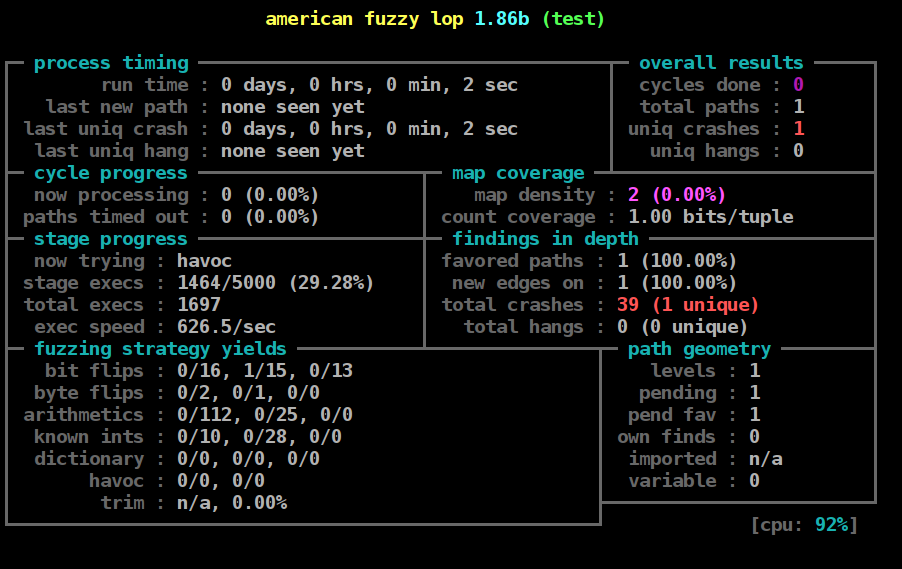
\includegraphics[width=0.9\linewidth]{images/American_fuzzy_lop's_afl-fuzz_running_on_a_test_program}
	\caption{AFL fuzzer}
	\label{fig:americanfuzzylopsafl-fuzzrunningonatestprogram}
\end{figure}

Furthermore, boofuzz is a Python-based fuzzing library most commonly used for protocol fuzzing. As such, it does not require code instrumentation to function. Instead, it supports building blueprints of protocols to be fuzzed using primitives and blocks. These can be thought of as representations of various common components of protocols, such as data types including strings, integers and bytes, but also other common features, such as length fields, delimiters and checksums. These allow users to specify protocol requests to be sent to the \ac{sut} and explicitly mark which portions of the request should be fuzzed via settings in the primitives. Possible settings on a per primitive/block level include the maximum length of data to be generated while fuzzing and also if the element in question should be fuzzed at all, or just be left at a default values. The option to define which parts of a protocol will be fuzzed at a field-by-field level gives boofuzz a high degree of flexibility. The exact fuzz data generated by the framework depends on the used blocks and settings, and then creates mutations based on the specified protocol structure. For example, a string primitive uses a list of many ``bad'' strings as a basis for mutation, which it then concatenates, repeats and otherwise mutates. Additionally, the \ac{sut} can be monitored for crashes and other unexpected behavior and the framework can furthermore be instructed to restart or reset the \ac{sut} when needed. In this paper, we use boofuzz primitives to generate our values for fuzzing, as detailed in Chapter \ref{chap:Fuzzing}.

\begin{figure}
	\centering
	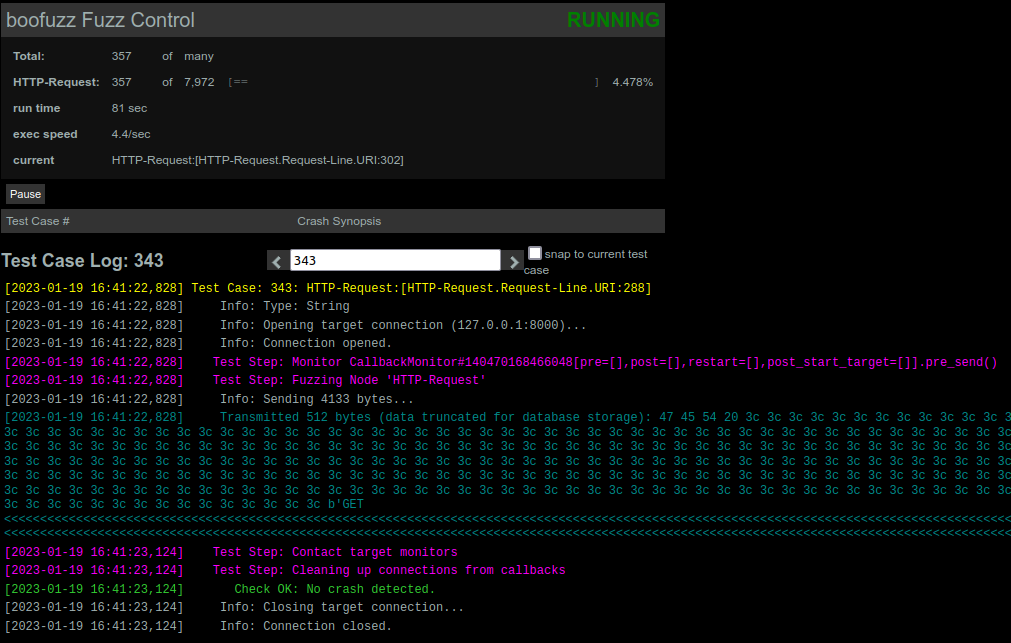
\includegraphics[width=0.9\linewidth]{images/boofuzz_control_center}
	\caption{Boofuzz fuzzer}
	\label{fig:boofuzzcontrolcenter}
\end{figure}

\newpage
\section{IPsec}
\ac{vpn}s are used to extend and or connect private networks across an insecure channel (usually the public internet). They can be used, e.g. to gain additional privacy from prying eyes such as Internet Server Providers, access to region-locked online content or secure remote access to company networks. Many different \ac{vpn} protocols exist, including PPTP, OpenVPN and Wireguard. Internet Protocol Security (\ac{ipsec}), is a \ac{vpn} layer 3 protocol suite used to securely communicate over an insecure channel. It is based on three sub-protocols, the \ac{ike} protocol, the \ac{ah} protocol and the \ac{esp} protocol. \ac{ike} is mainly used to handle authentication and to securely exchange as well as manage keys. Following a successful \ac{ike} round, either \ac{ah} or \ac{esp} is used to send packets securely between parties. The main difference between \ac{ah} and \ac{esp} is that \ac{ah} only ensures the integrity and authenticity of messages while \ac{esp} also ensures their confidentiality through encryption.

\begin{figure}[H]
\begin{centering}
	\begin{tikzpicture}[scale=1]
		\draw (-3,0) -- (-3,-9.2) (3,0) -- (3,-9.2);
		\node at (-3,.3) {Initiator};
		\node at (3,.3) {Responder};
		\draw[->] (-3,-1) -- node[midway,above] {ISAKMP SA \{proposals\}} (3,-1);
		\draw[<-] (-3,-2) -- node[midway,above] {ISAKMP SA \{proposal\}} (3,-2);
		\draw[->] (-3,-3) -- node[midway,above] {KE $\{pkey_i, nonce_i\}$} (3,-3);
		\draw[<-] (-3,-4) -- node[midway,above] {KE $\{pkey_r, nonce_r\}$} (3,-4);
		\draw[->] (-3,-5) -- node[midway,above] {AUTH $\{hash_i\}$} (3,-5);
		\draw[<-] (-3,-6) -- node[midway,above] {AUTH $\{hash_r\}$} (3,-6);
		\draw[->] (-3,-7) -- node[midway,above] {IPSEC SA \{proposals\}} (3,-7);
		\draw[<-] (-3,-8) -- node[midway,above] {IPSEC SA \{proposal\}} (3,-8);
		\draw[->] (-3,-9) -- node[midway,above] {ACK} (3,-9);
	\end{tikzpicture}
	\caption{IKEv1 between two parties}
	\label{fig:IKEv1}
\end{centering}
\end{figure}

The \ac{ike}v1 protocol works in two main phases, both relying on the \ac{isakmp}. Additionally, phase one can be configured to proceed in either Main Mode or Aggressive Mode. A typical exchange between two parties, an initiator (e.g. an employee connecting to a company network) and a responder (e.g. a company VPN server), using Main Mode for phase one and \ac{psk} authentication, can be seen in Figure \ref{fig:IKEv1}. In contrast, aggressive mode reduces the number of packets in phase one to only three. While faster, this method is considered to be less secure, as the authentication hashes are sent in clear text. In phase one (Main Mode), the initiator begins by sending a \ac{sa} to the responder. A \ac{sa} essentially details important security attributes required for a connection such as the encryption algorithm and key-size to use, as well as the authentication method and the used hashing algorithm. These options are bundled in containers called proposals, with each proposal describing a possible security configuration. While the initiator can send multiple proposals to give the responder more options to choose from, the responder must answer with only one proposal, provided both parties can agree upon one of the suggested proposals. This initial communication is denoted as \emph{ISAKMP SA} in Figure~\ref{fig:IKEv1} and also exchanges initiator/responder cookies, tokens used as identifiers for the remainder of the connection. Subsequently, the two parties perform a Diffie-Hellman key exchange, denoted as \emph{KE}, with the public key shorted to $pkey$, and send each other nonces used to generate a shared secret key \texttt{SKEYID} as detailed in Listing~\ref{lst:keying}. Here, \texttt{PSK} refers to the pre-shared key, \texttt{Ni/Nr} to the initiator/responder nonce and \texttt{CKY-I/CKY-R} to the initiator/responder identifier cookie. The symbol ``|'' is used to signify concatenation of bytes, not a logical or. Note that \ac{ike}v1 allows using various different authentication modes aside from PSK, including public key encryption and digital signatures. \texttt{SKEYID} is used as a seed key for all further session keys \texttt{SKEYID\_d}, \texttt{SKEYID\_a}, \texttt{SKEYID\_e}, with $g^{xy}$ referring to the previously calculated shared Diffie-Hellman secret and \texttt{prf} to a pseudo-random function (in our case, HMAC). 0, 1 and 2 are constants used to ensure that the resulting key material is different and unique for each type of key. Following a successful key exchange, all further messages of phase one and two are encrypted using a key derived from \texttt{SKEYID\_e} and \texttt{SKEYID\_a} for authentication. Note that the length of the actual encryption key depends on the used encryption algorithm, and is generated by concatenating hashes of \texttt{SKEYID\_e} and trimming the result until the desired length has been reached. This allows for the \texttt{SKEYID\_e} key to be used to generate arbitrary-length encryption keys. Finally, in the last section of phase one \emph{AUTH}, both parties exchange and verify hashes to confirm the key generation was successful. Once verification succeeds, a secure channel is created and used for phase two communication. If phase one uses Aggressive Mode, then only three packets are needed to reach phase two. While quicker, the downside of Aggressive Mode is that the communication of the hashed authentication material happens without encryption. This means, that using short \acp{psk} in combination with Aggressive Mode is inherently insecure, as the unencrypted hashes are vulnerable to brute-force attacks provided a short key-size~\footnote{\url{https://nvd.nist.gov/vuln/detail/CVE-2018-5389}}. The shorter phase two (Quick Mode) begins with another \ac{sa} exchange, labeled with \emph{IPSEC SA} in Figure~\ref{fig:IKEv1}. This time, however, the \ac{sa} describes the security parameters of the ensuing \ac{esp}/\ac{ah} communication and the data is sent authenticated and encrypted using the cryptographic material calculated in phase one. This is followed by a single acknowledge message, \emph{ACK}, from the initiator to confirm the agreed upon proposal. After the acknowledgment, all further communication is done via \ac{esp}/\ac{ah} packets, using \emph{SKEYID\_d} as keying material.

\begin{lstlisting}[float=ht, caption=IKE Keying, label=lst:keying]
	# For pre-shared keys: 
	SKEYID = prf(PSK, Ni_b | Nr_b)
	
	# to encrypt non-ISAKMP messages (ESP)
	SKEYID_d = prf(SKEYID, g^xy | CKY-I | CKY-R | 0)
	
	# to authenticate ISAKMP messages
	SKEYID_a = prf(SKEYID, SKEYID_d | g^xy | CKY-I | CKY-R | 1)
	
	# for further encryption of ISAKMP messages in phase two
	SKEYID_e = prf(SKEYID, SKEYID_a | g^xy | CKY-I | CKY-R | 2)
\end{lstlisting}

In addition to the packets shown in Figure~\ref{fig:IKEv1}, \ac{ike}v1 also specifies and uses so called \ac{isakmp} Informational Exchanges. Informational exchanges in \ac{ike}v1 are used to send \ac{isakmp} \emph{Notify} or \ac{isakmp} \emph{Delete} payloads. Following the key exchange in phase one, all Informational Exchanges are sent encrypted and authenticated. Prior, they are sent in plain. \ac{isakmp} \emph{Notify} payloads are used to transmit various error and success codes, as well as for keep-alive messages. \ac{isakmp} \emph{Delete} is used to inform the other communication partner, that a \ac{sa} has been deleted locally and request that they do the same, effectively closing a connection. 

Compared to other protocols, \ac{ipsec} offers a high degree of customizability, allowing it to be fitted for many use cases. However, in a cryptographic evaluation of the protocol, Ferguson and Schneier \textcite{ferguson1999cryptographic} criticize the complexity arising from the high degree of customizability as the biggest weakness of \ac{ipsec}. To address its main criticism, \ac{ipsec}-\ac{ike}v2 was introduced in RFC 7296 to replace \ac{ike}v1 \cite{kaufman2014internet}. Nevertheless, \ac{ipsec}-\ac{ike}v1 is still in wide-spread use to this day, with the largest router producer in Germany, AVM, still only supporting \ac{ike}v1 in their routers \cite{avm2022}. We use \ac{ipsec}-\ac{ike}v1 with Main Mode and \ac{esp} in this paper and focus on the \ac{ike} protocol as it is the most interesting from an AAL and security standpoint. % this part could maybe be moved to the introduction, not sure
			% Preliminary work: 7-10 pages
	
	% Part 2 Original Work
	
	\cleardoublepage
	%----------------------------------------------------------------
%
%  File    :  vpn_learning.tex
%
%  Author  :  Keith Andrews, IICM, TU Graz, Austria
% 
%  Created :  22 Feb 96
% 
%  Changed :  19 Feb 2004
% 
%----------------------------------------------------------------

\chapter{Model Learning}

\label{chap:Learning}

This chapter covers the learning and experiment setup. It showcases the many steps needed to learn the model of an \ac{ipsec} server, highlighting various design decisions. Additionally, implementation problems and our proposed solutions are discussed and presented. As until now we have been discussing learning algorithms from a theoretical standpoint, we will begin with a brief definition of automata learning terminology to use going forward that better suits the task of learning a reactive system. 

The goal of our learning setup is to learn a Mealy machine that models the \ac{sul}. We refer to it as the \textit{learned model}, or simply \textit{model} and \textit{automaton} interchangeably. To this end, we employ a learning algorithm, which requires an input alphabet $\Sigma$ of packets that are understood by the \ac{sul}. We refer to individual elements of the input alphabet as \textit{inputs}, whereas we refer to a chain of (multiple) inputs as an \textit{input sequence}. Each input of an input sequence will be executed on the \ac{sul} subsequently. We refer to one execution of our learning program as one learning attempt. A successful learning attempt is one that results in a correct behavioral model of the \ac{sul}. As we are working with Mealy machines, the term \textit{output query} is used instead of membership query.

% Basic Model-Learning workflow
\section{Learning Setup} \label{subsec:learningenv}% half - quarter page
The models of two separate \ac{ipsec} implementations were learned, namely behavioral models of strongSwan and libreswan \ac{ipsec} server implementations. The \ac{ipsec} servers were installed and setup on the responder \ac{vm}, as detailed in Chapter~\ref{chap:Setup}. They were configured to listen for incoming connections from the initiator \ac{vm}, which are generated by our learning setup. On a high level, our learning framework consists of four main parts, as shown in Figure \ref{fig:AALSetup}. These are the learning algorithm, the custom mapper, the communication interface and the \ac{sul}. The learning algorithm handles the actual learning via the $L^*$ or $KV$ algorithm. This is in large part done using the Python automata learning library \textsc{AALpy}~\cite{software:aalpy} version 1.2.9. \textsc{AALpy} supports deterministic, non-deterministic and stochastic automata, including support for various formalisms for each automata type. We chose deterministic Mealy machines to describe the \ac{ipsec} server, as they are commonly used to model reactive systems. However, learning automata with \textsc{AALpy} follows the same basic process, regardless of the type of automata used.

The custom mapper makes up a large portion of our work and is used to convert between abstract inputs and actual \ac{isakmp} packets, using the packet manipulation library Scapy\footnote{\url{https://scapy.net/}}, version 2.4.5. Scapy was used to parse and create \ac{isakmp} packets, which are used by the communication interface to communicate with the \ac{ipsec} server. Significant effort was put into expanding the \ac{isakmp} Scapy module to support all packets required for \ac{ipsec}, as the module lacked many features out-of-the-box. The provided Python script, \emph{IPSEC\_IKEv1\_SUL}\footnote{\TODO{GITHUB LINK}} demonstrates how \textsc{AALpy} can be used in conjunction with our custom mapper and communication interface to communicate with, and learn the model of an \ac{ipsec} server. What follows, is a more detailed look at how the individual parts of the learning framework work together to learn the model of an \ac{ipsec} server.

\begin{figure}[h]
	\begin{tikzpicture} 
		\node (n1) [draw, minimum width=7em, minimum height=3.5em, align=left] at (0,1) {~Learning\\~Algorithm};
		\node (n2) [draw, minimum width=7em, minimum height=3.5em, align=left] at (4.4,1) {~Mapper};
		\node(n3) [draw, minimum width=7em, minimum height=3.5em,  align=left] at (8.8,1) {~Interface\\~(Initiator)};
		\node(n4) [draw, minimum width=7em, minimum height=3.5em,  align=left] at (13.2,1) {~SUL\\~(Responder)};
		\draw [->] ($(n1)+(3.5em,+0.5em)$) -> ($(n2)+(-3.5em,+0.5em)$) node[midway,above,align=center] {\scriptsize~Abstract\\\scriptsize~Input};
		\draw [->] ($(n2)+(-3.5em,-0.5em)$) -> ($(n1)+(3.5em,-0.5em)$) node[midway,below,align=center] {\scriptsize~Abstract\\\scriptsize~Output};
		
		\draw [->] ($(n2)+(3.5em,+0.5em)$) -> ($(n3)+(-3.5em,+0.5em)$) node[midway,above,align=center] {\scriptsize~Concrete\\\scriptsize~Input};
		\draw [->] ($(n3)+(-3.5em,-0.5em)$) -> ($(n2)+(3.5em,-0.5em)$) node[midway,below,align=center] {\scriptsize~Concrete\\\scriptsize~Output};
		
		\draw [<->] (n3) -> (n4) node[midway,above,align=center] {\scriptsize~UDP};
	\end{tikzpicture} 
	\caption{Automata Learning Setup}
	\label{fig:AALSetup}
\end{figure}

Figure \ref{fig:AALSetup}, adapted from Tappler et al.~\cite{tappler2017}, gives an overview of the model learning process. To begin, the learning algorithm sends abstract inputs chosen from the input alphabet to the mapper class, which converts it to concrete inputs. In other words, the mapper class converts between sequences of abstract and concrete inputs. The concrete inputs are then sent to the \ac{sul}, by means of the communication interface. In our case, the mapper class comprises the major portion of our work in the establishment of the learning framework and converts the abstract words into actual \ac{ipsec} packets that can be sent to the \ac{sul} Strongswan server via UDP packets. This alphabet abstraction step simplifies the learning process, as learning the model for all possible inputs of an \ac{ipsec} server would be tedious at best. Additionally, the separation between abstract and concrete inputs/outputs allows for easy future modifications to the message implementations, including fuzzing support, as well as increasing the readability of our code. 

\begin{table}[h]
	\centering
	\begin{tabular}{|l|l|}
		\hline
		\rowcolor[HTML]{DAE8FC} 
		\hline
		\multicolumn{1}{|l|}{\cellcolor[HTML]{DAE8FC}\textbf{Protocol}} & \multicolumn{1}{l|}{\cellcolor[HTML]{DAE8FC}\textbf{Input Alphabet}} \\ \hline
		ISAKMP SA                                                       & sa\_main                                                             \\
		KE                                                              & key\_ex\_main                                                        \\
		AUTH                                                            & authenticate                                                         \\
		IPSEC SA                                                        & sa\_quick                                                            \\
		ACK                                                             & ack\_quick                                                           \\ \hline
	\end{tabular}
	\caption{Mapping protocol to input alphabet names}
	\label{tab:map_prot_ia}
\end{table}

To begin learning an automaton with \textsc{AALpy}, one must first choose a suitable input alphabet encompassing the language known by the server, as well as the learning algorithm to be used. Our chosen input alphabet corresponds to the \ac{ike}v1 protocol messages shown in Figure \ref{fig:IKEv1}. The protocol messages map to abstract inputs of the input alphabet as shown in Table~\ref{tab:map_prot_ia}. We use both the $L^*$ and $KV$ algorithms for learning with a state prefix equivalence oracle that provides state-coverage by means of random walks started from each state. The equivalence oracle is used by the chosen learning algorithm to test for conformance between the current hypothesis and the \ac{sul}, giving either a counterexample on failure, or confirmation that the \ac{sul} has been learned successfully. This corresponds to an equivalence query. Additionally, several optional \textsc{AALpy} features were enabled, including caching and non-determinism checks to improve the learning process. An overview of the relevant learning algorithm initialization code can be seen in Listing \ref{lst:eqcode}. Line 3 shows the used input alphabet, Line 4 the used equivalence oracle and Line 5 the used learning algorithm. Both the equivalence oracle and learning algorithm take the input alphabet and an object representing an interface to the \ac{sul} as parameters, were the \ac{sul} interface is defined as shown below in \ref{lst:sulinterface} and can execute inputs on, as well as reset the the actual \ac{sul}. The equivalence oracle is also passed as a parameter to the learning algorithm with a few additional optional parameters specifying the type of automaton to learn and enabling non-determinism checking and caching.

\begin{lstlisting}[float=h, caption=Equivalence Query code, label=lst:eqcode, language=python]
	# Code example detailing AAL with AALpy
	
	input_al = ['sa_main', 'key_ex_main', 'authenticate', 'sa_quick', 
	'ack_quick']
	eq_oracle = StatePrefixEqOracle(input_al, sul, walks_per_state=10, walk_len=10)
	learned_ipsec = run_Lstar(input_al, sul, eq_oracle=eq_oracle, automaton_type='mealy', cache_and_non_det_check=True)
	
\end{lstlisting}

The \ac{sul} interface defines the \emph{step} and \emph{reset} methods, as can be seen in Listing \ref{lst:sulinterface}. \emph{step}, seen in Line 3, is used to execute input actions. \emph{reset}, show in lines 8-12, reverts the \ac{sul} to an initial state. An output query is a sequence of inputs executed on the \ac{sul}. Every input sequence is executed starting from an initial state, hence the need for a \emph{reset} method. Used in combination, \emph{step} and \emph{reset} allow asking output queries to the \ac{sul}. \emph{pre} is called before each output query and \emph{post} afterwards. The abstract input chosen from the input alphabet is passed on to the mapper class for further processing. Line 4 shows how a function, corresponding to the abstract input, is called in the mapper class and the return value (abstract output) is passed on to the learning algorithm. \\

\begin{lstlisting}[float=h, caption=SUL interface, label=lst:sulinterface, language=python]
	# code excerpt from IPSEC_IKEv1_SUL.py
	
	def step(self, input):
		func = getattr(self.ipsec, input)
		ret = func()
		return ret
	
	def pre(self):
		self.ipsec.reset()
	
	def post(self):
		self.ipsec.delete()
\end{lstlisting}

The mapper class implements methods for each communication step in a typical \ac{ipsec}-\ac{ike}v1 exchange, as described in Section \ref{chap:Preliminaries}, but referred to by their input alphabet name according to Table~\ref{tab:map_prot_ia}. This includes methods for \emph{sa\_main}, \emph{key\_ex\_main}, \emph{authenticate}, \emph{sa\_quick}, \emph{ack\_quick} packets. Additionally, the mapper class supports \emph{DELETE} messages. The \emph{DELETE} message is special in that it actually sends two packets which is required to delete all existing connections to the Strongswan server. It is critical for the correct functioning of \emph{reset} that this input is executed correctly, hence it requires the \ac{sul} state be checked after execution, which is not feasible during learning. For these two reasons, it was mostly left out of the learning process. Furthermore, the mapper class contains a variety of helper functions used to handle the decryption and encryption of packets as well as parse received informational messages. Informational messages are mainly used in \ac{ipsec} to return error codes when something goes wrong. To illustrate our mapper class, (simplified) excerpts from the \emph{sa\_main} method are shown in Listing \ref{lst:mapper1}. It shows how a Scapy packet is constructed out of many different individually configurable layers and fields, allowing for a high degree of flexibility and customizability. Line 5 shows how an \ac{isakmp} transform is created, encompassing various security parameters. This transform is packed into a \ac{isakmp} proposal packet first and then the resulting packet is packet into an \ac{isakmp} \ac{sa} packet in Line 6. The \ac{sa} packet is appended to a generic top level \ac{isakmp} packet in Line 8. In Line 9 the \ac{isakmp} packet is sent to the \ac{sul} and its response (if any) is received. The connection manager, initialized as \texttt{self.\_conn}, handles the actual sending and receiving logic and returns the server response already converted into a matching Scapy object. The Scapy response object then undergoes a retransmission check and is then parsed with relevant data being used to update local values, as indicated in lines 11-16.

\begin{lstlisting}[float=h, caption=Excerpt of sa\_main method code, label=lst:mapper1, language=python]
	# code excerpt from IPSEC_MAPPER.py
	
	def sa_main(self, ...):
	...
	tf = [('Encryption', 'AES-CBC'), ('KeyLength', 256), ('Hash', 'SHA'), ('GroupDesc', '1024MODPgr'), ('Authentication', 'PSK'), ('LifeDuration', 28800)]
	sa_body_init = ISAKMP_payload_SA(prop=ISAKMP_payload_Proposal(trans_nb=1, trans=ISAKMP_payload_Transform(num=1, transforms=tf)))
	
	policy_neg = ISAKMP(init_cookie=cookie_i, next_payload=1, exch_type=2)/sa_body_init
	resp = self._conn.send_recv_data(policy_neg)
	
	if (ret := self.get_retransmission(resp)): 
	# retransmission handling
	...
	
	# Response handling (checks response code, decrypts if necessary, updates relevant local values)
	...
\end{lstlisting}

The \ac{ipsec} packets generated by the mapper class are passed on to our communication class, which acts as an interface for the \ac{sul} and handles all incoming and outgoing UDP communication. Additionally, it parses responses from the \ac{sul} into valid Scapy packets and passes them on to the mapper class. The mapper class then parses the received Scapy packets and returns an abstract output code representing the received data to the learning algorithm. This code corresponds to the type of received message, or in the case of an error response (informational message), the error type. For fuzzing purposes, several common error types were grouped together into categories and the error category was used as the return value. Finally, the abstract error codes are returned to the learning algorithm which uses it update its internal data structures and improve its understanding of the \ac{sul} by updating the model. \\

\section{Design Decisions and Problems} \label{subsec:design}
% Design details advantages and disadvantages --> problems and solutions (2-3p)
We use the Python library Scapy to construct \ac{isakmp} packets as required by the \ac{ike}v1 protocol. More exactly, we use the \ac{isakmp} package that defines a generic top-level \ac{isakmp} package as well as several more specific payloads that it can contain. Parsing was made more difficult by the fact that Scapy does not support/implement all the packets required by \ac{ipsec}-\ac{ike}v1. To solve this problem, we implemented all missing packets in the Scapy \ac{isakmp} class and used this modified version. Specifically, we added support for \ac{isakmp} Informational packets, including resolving all commonly supported error codes, \ac{isakmp} Delete packets, NAT-D, additional SA attributes for \ac{isakmp} and ESP. Additionally, we improved the \ac{isakmp} Transform, Proposal and ID packets. In addition to all the \ac{isakmp} packets, our chosen automata learning algorithms require a \ac{sul} reset method to be able to return to an initial starting point after each query. Due to design differences between strongSwan and libreswan, we were forced to implement this reset method differently for the two \ac{ipsec} servers. For strongSwan, we implement reset using a combination of the \ac{isakmp} \emph{DELETE} request and general \ac{isakmp} informational error messages. While \emph{DELETE} alone works for established connections in phase two of \ac{ike}, we require informational error messages to trigger a reset in phase one, as delete does not work here sufficiently. On the other hand, libreswan does not allow remote resetting of phase one connections at all, so here we were forced to implement the reset method by sending \texttt{ipsec restart} commands via a SSH connection directly to the \ac{ipsec} manager backend. This adds an additional separate medium of communication, outside the existing protocol stack, potentially skewing runtime measurements. Therefore, the strongSwan implementation was used for most benchmarks, as there, all messages sent were part of the \ac{ipsec} protocol stack and the reset method does not depend on having root access to the \ac{sut} (as is unlikely in a black-box scenario).

Each concrete mapping function in our mapper class can be run with a standard configuration, or with arbitrary values for the respective fields of the resulting packet. This allows us to learn different variations of the \ac{ipsec} servers. For example, our mapper class allows us to very easily switch between learning a server model when presented with valid inputs, and the model of a server when introduced to invalid, malformed messages in combination with valid ones. Additionally, this design of the mapper functions will make fuzz testing specific protocol messages quite simple. The model of a server presented with malformed inputs will serve as the basis for future model-based fuzz testing and can be seen in Chapter~\ref{chap:Evaluation}.

As inputs will be sent in many different, potentially unusual, combinations during learning, we require a robust framework that correctly handles the encryption and decryption of \ac{ipsec} messages. For key management, we simply store the current base-keys but keep track of \acp{iv} on a per \ac{mid} basis. Additionally, we keep track of the M-IDs of server responses to detect and handle retransmissions of old messages. As libreswan also sends retransmissions of phase one messages, we additionally have to store identifying information (nonces, hashes, etc.) to be able to match retransmissions to past messages, as phase one messages all have the same \ac{mid} of zero.
Each request, we store the response for use in the next message and update affected key material as needed. Most notably, the \acp{iv} are updated almost every request and differ between M-IDs. Informational requests also handle their \acp{iv} separately from other message types. For each request that we send, if available, we try to parse the response, decrypting it if necessary and resetting or adjusting our internal variables as required to match the server. To keep track of all the different \acp{mid}, we use a Python dictionary to map \acp{mid} to relevant keying and \ac{iv} information. Usually, \acp{iv} are updated to the last encrypted block of the most recently sent or received message, though this behavior varies slightly between phases and for informational messages. Keeping track of \acp{iv} is required to continuously be able to parse encrypted server responses and extract meaningful information. Implementation of the mapper class, in particular encryption and decryption functionality, was hindered at times by unclear RFC-specifications, but this was overcome by manually comparing packet dumps and \ac{ipsec} server logs to fix errors, as detailed in Chapter~\ref{chap:Setup}.\\

To ensure that we receive all responses, we add a timed wait for each server response. In the case of no response arriving during the wait, we directly return an empty \textit{None} response and need no further handling. Otherwise, we check the response \ac{mid} against our list of previous \acp{mid} to detect retransmissions. A retransmission is when the server returns a previously returned message in response to a new request. In this case, the retransmission \ac{mid} (or other identifier in the case of libreswan phase one messages) is the same for both responses. Our retransmission handling is covered in more detail in Section~\ref{sec:nondet}. If a retransmission is detected, depending on the configured retransmission-handling rule, it is either ignored or the corresponding previous response is returned. To save some time when not ignoring retransmissions, we keep a dictionary mapping \acp{mid} to their parsed response codes, allowing us to skip the parsing stage for retransmitted messages and return the saved previously parsed response directly. If no retransmission is detected, we check that the message type matches the expected one and if so, parse the message further to update local values and extract a response code. If the message type does not match, it is usually an informational message, indicating some sort of error. In this case, we decrypt the message using the corresponding parameters (as they are calculated and saved differently for informational messages), and return a code indicating the error being reported. Finally, we catch and log unimplemented message types, but this case should not occur during learning and is implemented mainly for later fuzzing.

Since testing and automata learning can be a very time-intensive process, we implemented several performance improvements to speed up the learning process. First, we reduced the timeouts down to a minimal amount needed to still get deterministic results. Next, we categorized the server informational responses according to their severity and impact and then grouped the most common ones together under the same abstract response code. This decreased the amount of states that had to be learned at the cost of some informational loss. However, since any deviations or non-deterministic behavior would have been caught by the learning framework, we are confident that no important information was lost. Finally we switched out the $L^*$ learning algorithm for $KV$, as $KV$ can be more performative for learning environments where output queries are expensive operations. As \ac{ike}v1 is a networks protocol with quite a bit of communication in each phase and we additionally have to implement small timeouts to wait for the server, each individual output query can take several seconds. With hundreds of output queries required to learn the \ac{ipsec} server, this results in a lot of time spent running the algorithm. Consequently, any decrease to the amount of output queries should, in theory, lead to an overall decrease in runtime. Since \textsc{AALpy} supports the $KV$ algorithm, switching between the two learning algorithms is as easy as setting a simple flag as shown in line three of Listing \ref{lst:newalg} below. The $KV$ algorithm required less output queries to learn the \ac{sul} and consequently significantly improved the speed at which models could be learned. The detailed comparison of runtime statistics between $L^*$ and $KV$ can be found in Chapter \ref{chap:Evaluation}.

\begin{lstlisting}[float=ht, caption=Switching Learning Algorithms, label=lst:newalg, language=python]
	# code excerpt from IPSEC_IKEv1_SUL.py
	
	if kv:
	learned_ipsec, info = run_KV(input_al, sul, eq_oracle, automaton_type='mealy', cex_processing='rs')
	else:
	learned_ipsec, info = run_Lstar(input_al, sul, eq_oracle=eq_oracle, automaton_type='mealy', cache_and_non_det_check=True)
\end{lstlisting}


% non-determinism fixes
\section{Combating Non-determinism} \label{sec:nondet}
Despite many precautions taken to create a disturbance-free learning environment, as detailed in Chapter~\ref{chap:Setup}, the \ac{ipsec} servers still exhibited non-deterministic behavior, resulting in variance among the learned models. While the majority of learned models were identical, the outliers were significantly different, having differing amounts of states and transitions between them. To help decrease the remaining non-deterministic behavior, additional timeouts were added to all requests in order to give the server more time to correctly work through all incoming requests. This measure helped further decrease the amount of outlying automata learned, however it did not fully fix the issue. Examination of the outliers led to the discovery that all outlying behavior was concentrated around so-called retransmissions. Essentially, the \ac{ike} specification allows for previous messages to be retransmitted if deemed useful. A possible trigger could be the final message of an \ac{ike} exchange being skipped / lost. For example, if instead of an \emph{AUTH} message, the server receives a phase two \emph{IPSEC SA} message, the server would not know if it missed a message or if their was an error on the other parties side. According to the \ac{isakmp} specification in RFC 2408~\cite{rfc:isakmp}, the handling of this situation is unspecified, leaving the exact handling up to the implementations, however two possible methods are proposed. Firstly, if the \emph{IPSEC SA} message can be verified somehow to be correct, the server may ignore the missing message and continue as is. Secondly, the server could retransmit the message prior to the missing one to force the other party to respond in kind. Strongswan appears to implement these retransmissions and due to internal timeouts of connections, they seem to trigger in a not-quite-deterministic fashion in phase two of \ac{ipsec} \ac{ike}v1 protocol. libreswan also implements retransmissions, but here they also occur in phase one, forcing us to identify the messages in question in other ways (nonces, hashes, etc.).

While interesting for fingerprinting, as certain models were learned with a much higher frequency than the outliers and they contain a lot of information, a deterministic model was required to serve as a base case for model-based fuzzing. Therefore, checks were added in our mapper to allow for the ignoring of retransmissions. The retransmission-filtering can be easily enabled or disabled through a simple flag and works by checking the message ID of incoming server responses against a list of previous message IDs (excluding zero, as it is the default message ID for phase one) and other identifying information for libreswan phase one retransmissions. If a repeated message is found, it is flagged as a retransmission and depending on the current filtering rule, ignored. With this addition, non-deterministic behavior no longer occurred, allowing the learning of very clean models, as shown in Chapter~\ref{chap:Evaluation}, Figure \ref{fig:reference} and Figure \TODO{ADD REF TO LIBRESWAN REF MODEL!}. As an additional method of dealing with non-determinism problems, but still keeping retransmissions, non-determinism errors can be caught as they occur and the offending queries repeated several times. If upon the first rerun the non-determinism does not occur again, the existing value can be accepted as the correct one. If however, the non-determinism errors persist for a set amount of repetitions with the same constant server response, it is likely, that the original saved response was incorrect and it can be updated to the new response. However, this method heavily impacts runtime performance, as many queries have to be repeatedly sent. As retransmissions are inherently non-deterministic and we need deterministic models for fuzzing, we decided to use mainly the filtering approach for our models. With the non-determinism correcting added, the automata learning works without non-determinism errors and the learned models are consistent with one another.
		% Automata Learning setup and overview described as in shortpaper, then design and implementation, 
	
	\cleardoublepage			% setup of Fuzzing, then implementation  then maaaaybe Fingerprinting and then implementation
	%----------------------------------------------------------------
%
%  File    :  vpn_fuzzing.tex
%
%  Author  :  Benjamin Wunderling, TU Graz, Austria
% 
%  Created :  22 Feb 96
% 
%  Changed :  19 Feb 2004
% 
%----------------------------------------------------------------

\chapter{Fuzzing}

\label{chap:Fuzzing}

\section{Environment Setup} \label{sec:environment}
% describe VMs, IPsec server software, configuration etc
We ran all our fuzzing tests in the same virtual network setup we used for our automata learning, on the same Ubuntu 22.04 LTS distributions. We again designated one VM as the initiator which would send the fuzzed messages and the other one as the responder to create a typical client-server setup. All settings on the used VMs remained the same as while learning to ensure that no discrepancies were introduced by different environment settings. The system under test (SUT) was also the same Strongswan server used for learning. 

\subsection{Adapting the Model} \label{subsec:adapting_model}
While we had already successfully learned a (deterministic) model of the SUL when exposed to expected inputs, this proved to be not particularly useful for model-based fuzzing, as each fuzz case would be treated as new behavior. Instead we learned a new model, again with retransmission-filtering enabled, but this time also with an expanded input alphabet. We added an erroneous version of each input letter that maps to an IKE packet with some sort of error or malformation, as shown in Listing \ref{lst:inputal_2}. The goal was to learn the behavior of the SUL when exposed to typical errors or malformed packets that could arise during fuzzing, to be able to filter away as much uninteresting information as possible and focus on more unusual behavior. An example of such a malformed packet could be an incorrect length field, a wrong hash value or simply an unsupported SA option. Since we had designed our mapper class in such a way as to allow for easy manipulation of packets, this was an easy change to implement. Some additional server responses had to be parsed correctly, but all in all, not much had to be changed. The resulting model can be seen in Figure \ref{fig:withfilterwitherrors} and was used as our reference model while testing.  

\begin{lstlisting}[float=h, caption=The updated input Alphabet, label=lst:inputal_2, numbers=none, language=python]
	# code excerpt from IPSEC_IKEv1_SUL.py
	
	input_al = ['sa_main', 'key_ex_main', 'authenticate', 'sa_quick', 'ack_quick', 'sa_main_err', 'key_ex_main_err', 'authenticate_err', 'sa_quick_err', 'ack_quick_err']
\end{lstlisting}


\subsection{Fuzzing Setup} \label{subsec:fuzz_setup}
% tools used
As we had already designed our mapper class in such a way as to allow for easy fuzzing, the only thing missing was a source of values to use for fuzzing. For this purpose, we used the open source fuzzing library boofuzz\footnote{https://github.com/jtpereyda/boofuzz}, which is a successor of the popular Sulley\footnote{https://github.com/OpenRCE/sulley} fuzzer. Additionally we implemented a very simple parser for the .dot files of the learned model, as well as a converter between .dot files and state machines.

% procedure --> 2 phases: p1 - prefiltering, p2 - boofuzz fuzz lists
The general procedure for model-based fuzzing is to fuzz the target system, while at the same time keeping track of the expected outputs on a reference model, to be able to identify new states and interesting behavior. While our fuzzer does follow this pattern, due to the IPsec-IKEv1 protocol being rather complicated, fuzzing every possible field would be an immense task that goes far beyond the scope of this masters thesis. Instead, we implemented several techniques to limit the amount of fuzzing to be done in a way that aims to still maximize the chances of discovering new states and potential bugs. 

Firstly, instead of fuzzing every possible field of the protocol, we instead chose 5-10 key fields from each packet that looked to be the most impactful and representative for that type of message. We focused on length fields, SA proposals and hashes / keys, but also added general fields, such as the responder / initiator cookies. All the chosen fields were added as parameters to their respective mapper class methods and default to their usual values. 

The next step was the run-generation phase in which we look to generate a set of runs consisting of input alphabet words, were one of the letters will be randomly chosen to be fuzzed. Our first idea was to go on random walks through the state machine and mirror the messages sent to the SUT as well, but the problem here at least for truely random walks was a lot of wasted queries in phase one and not enough state coverage in phase two. Therefore, since we had already generated a number of runs during model learning that guarantee state-coverage, we decided to simply repurpose those runs for fuzzing. The problem with this approach however, was that the resulting set of runs was rather large. So, in an effort to reduce the fuzzing space, we employed an additional filtering phase before the actual in-depth fuzzing. In this phase, we go through each run one by one and randomly designate one of its input alphabet letters as the fuzzing target. Then we test each parameter of that letter in the context of the run with a greatly reduced set of fuzz values and compare the results to the expected outcomes using our state machine. If new behaviour is found, the run and fuzz target passes the filtering. Runs in which no new behavior is discovered are discarded. This allows us to focus our resources on testing those configurations in which it is more likely to discover new behavior and therefore also bugs. 

Following the automatic filtering, we go over the results and manually check and remove / reduce the number of identical or not relevant cases. For example, we noticed that every run in which cookies were fuzzed led to new states, due to new cookies indicating a completely new connection and since we learned the model with static initiator cookies, this will always lead to a new state. 
Finally, we arrive at a list of 175 runs, compared to roughly ten times the number before filtering. The filtered list of runs can be found in Appendix TODO: APPENDIX.


% TODO: improvements for run-generation, potentially refine the model with new info


Phase two, take the (hopefully reduced) list of interesting runs and fuzz targets on those runs and apply actual in-depth fuzzing using boofuzz to generate our fuzz-cases for all but the most complicated of parameters

TODO: Diagram for fuzzing process
Placeholder for grafic
p\\
p\\
p\\
p\\
p\\
p\\
p\\
p\\
p\\
p\\
p\\
p\\
p\\
p\\
p\\
p\\
p\\
p\\

	
	\cleardoublepage
	%----------------------------------------------------------------
%
%  File    :  vpn_evaluation.tex
%
%  Author  :  Benjamin Wunderling, TU Graz, Austria
% 
%----------------------------------------------------------------

\chapter{Evaluation} \label{chap:Evaluation}

This chapter presents the results of our model learning and model-based fuzzing for \ac{ipsec}-\ac{ike}v1. Model learning results are presented in Section \ref{sec:learnresults}, beginning with the models learned without retransmission-filtering. All model learning and testing took place in a virtual environment using two VirtualBox 6.1 \acp{vm} running standard Ubuntu 22.04 LTS distributions, as described in \ref{chap:Setup}. Next, models of both examined \ac{ipsec} implementations, with retransmission-filtering enabled, are presented and discussed, highlighting differences between the models of the two \ac{ipsec} implementations. The presentation of learned models is followed by a comparison of the two used learning algorithms, $L^*$ and $KV$, as well as the discussion of a library error found during learning. Finally, the fuzzing results for both \ac{ipsec} servers are presented and discussed in Section \ref{sec:fuzzresults}, comparing the various methods of input-sequence generation introduced in Chapter~\ref{chap:Fuzzing}.

\iffalse
\section{Environment Setup} \label{sec:env}
% describe VMs, IPsec server software, configuration etc
All model learning and testing took place in a virtual environment using two VirtualBox 6.1 \acp{vm} running standard Ubuntu 22.04 LTS distributions. Both \acp{vm} were allotted \SI{4}{\giga\byte} of memory and one CPU core. All inter-\ac{vm} communication took place in an isolated virtual network to eliminate possible external influences. During learning and fuzzing, all power saving options and similar potential causes of disruptions were disabled. Additionally, the \ac{ipsec} server was restarted before each learning attempt to ensure identical starting conditions. One \ac{vm} was designated as the initiator and one as the responder to create a typical client-server setup. We chose the open source \ac{ipsec} implementation strongSwan~\cite{software:strongSwan} as our \ac{sul}. The strongSwan server was installed on the responder \ac{vm} and set to listen for incoming connections from the initiator \ac{vm}. We used the strongSwan version US.9.5/K5.15.0-25-generic, installed using the default Ubuntu package manager, apt. The strongSwan server was configured to use \acp{psk} for authentication and default recommended security settings. Additionally, it was configured to allow unencrypted notification messages, which were used to reset the connection during the learning process. Our strongSwan configuration files can be found in Appendix~\ref{app::dot}. The Python library \textsc{AALpy}~\cite{software:aalpy} version 1.2.9 was used in conjunction with the packet manipulation library Scapy\footnote{\url{https://scapy.net/}}, version 2.4.5, in order to learn a model of the \ac{sut}. Significant effort was put into expanding the \ac{isakmp} Scapy module to support all packets required for \ac{ipsec} as the module lacked many features out-of-the-box. The provided Python script, \emph{IPSEC\_IKEv1\_SUL}\footnote{\url{https://github.com/benjowun/VPN-AL}}, demonstrates how \textsc{AALpy} can be used in conjunction with our custom mapper to communicate with and learn the model of an \ac{ipsec} server. Figure~\ref{fig:AALSetup} shows a typical learning attempt using two connected \acp{vm}. The right \ac{vm} shows the output of an underway learning attempt, while the left one shows the corresponding strongSwan server logs.
\fi

\section{Learning Results} \label{sec:learnresults}
% section where we show and analyze reference and no filter models including model and statistics
Over the course of our work, we learned a variety of different models of both \ac{ipsec} servers, due to varying retransmission-handling settings and choices of the input alphabet. As our \ac{sul} had some issues with non-determinism while retransmissions were enabled, one major differentiating factor in our models is whether retransmission-filtering was enabled for the learning process. This had a significant impact on the resulting learned model, with the version without filtering boasting more than twice the number of states than the one with. Additionally, even when using the methods to combat non-determinism described in Section \ref{sec:nondet}, the resulting models still occasionally differed when not filtering out retransmissions. Therefore, the non-filtered models were not used for fuzzing, as a completely deterministic model was desired to serve as our baseline when fuzzing the \ac{sut}.

The following sections first introduce the most relevant metrics used to evaluate the learned models. Next, the two most commonly learned models without retransmission-filtering, both learned from a Linux strongSwan U5.9.5 server, are presented. Finally, models of both servers using the basic and extended input alphabets, with retransmission-filtering enabled, are presented. All models were learned using both the $KV$ and $L^*$ learning algorithms. Error codes have been simplified for better readability and DOT files of all models are provided in Appendix~\ref{app::dot}, as well as in the supplementary material\footnote{\url{https://github.com/benjowun/VPN-AL}}. Note that \textsc{AALpy} refers to output queries as membership queries.

\newpage

\subsection{Learning Metrics} \label{subsec:metrics}
The comparison of learned models and model learning algorithm performance in sections \ref{subsec:models} and \ref{subsec:comp_kv_lstar} is based largely on the following metrics, saved during the model learning process.

\subsubsection*{Steps}
Steps refers to the number of inputs executed on the \ac{sul}.

\subsubsection*{Queries}
Queries refers to the amount of queries sent during state exploration (output queries) or during conformance checking (equivalence queries). \textsc{AALpy} supports speeding up model learning by using caching to reduce the number of required output queries. 

\subsubsection*{Runtime}
Runtime refers to the time it took to learn the model. It is further split into state exploration and conformance checking runtimes. Runtime directly correlates to the number of steps and queries. When given in seconds, the runtime is rounded to the nearest second.


\subsection{Learned strongSwan Models} \label{subsec:models}
Figures \ref{fig:ret_case1} and \ref{fig:ret_case2} show the two most commonly learned strongSwan models when not filtering retransmissions. Roughly 80\% of all models learned without retransmission-filtering enabled resulted in one of these two models, which we will refer to as the common models. The other 20\% of models were a non-uniform assortment of outliers. 

Figure \ref{fig:reference} shows the clean base model learned from the strongSwan \ac{sul} with retransmission-filtering enabled. Figure \ref{fig:learnedmodellibresimple} shows the equivalent libreswan clean base model. The strongSwan reference model used for fuzzing is shown in Figure \ref{fig:withfilterwitherrors}, also learned with retransmission-filtering enabled, as well as an expanded input alphabet. Figure \ref{fig:learnedmodellibrereference} shows the equivalent libreswan fuzzing reference model.

The strongSwan runtimes of both learning algorithms for all four models are summarized in tables \ref{tab:runtime_summary_kv} and \ref{tab:runtime_summary_lstar}. All values are averages over multiple learning attempts. The libreswan runtimes were omitted from the statistics, as a workaround had to be used to reset the \ac{ipsec} host \ac{vm} between output queries, potentially skewing the results. The tables use the following abbreviations:

\begin{enumerate}
	\item States: The number of states in the learned model
	\item TT (s): Total time needed to learn the model (in seconds)
	\item TL (s): Time spent on state exploration (in seconds)
	\item TC (s): Time spent on conformance checking (in seconds)
	\item OQ: Number of output queries sent during the model learning
	\item CT: Size of the conformance testing suite, i.e. the number of performed conformance tests
\end{enumerate}
 

\subsubsection*{First Common Model}

The first common model, learned from the strongSwan server, is presented in Figure \ref{fig:ret_case1} and took approximately 52 minutes (3092 seconds) to learn with the $KV$ algorithm, spread over seven learning rounds. The model consists of ten states. Of the 52 minutes total, roughly half were used for state exploration/output queries and the other half for conformance checking, with conformance checking taking slightly longer (1501 vs 1591 seconds). 171 output queries were performed by the learning algorithm in 2047 steps, whereas 100 conformance tests were performed for equivalence checking in 1826 steps.

In contrast, when learned with the $L^*$ algorithm, model learning took almost 85 minutes (5094 seconds) over five learning rounds. Here, the split between state exploration and conformance checking was more distinct, with state exploration taking up approximately 68\% of the total runtime and conformance checking only requiring the remaining 32\% (3489 vs 1605 seconds). 462 output queries were required compared to the 171 of the $KV$ algorithm. Notably, the time needed for conformance checking remained largely the same between the two algorithms, however the difference in state exploration/output queries is quite large. This behavior is discussed in more detail in Section \ref{subsec:comp_kv_lstar}, which includes a statistical comparison of the two algorithms.

\begin{figure}[ht]
	\vspace*{\fill}
	\noindent
	\hspace*{-5.5\oddsidemargin}%
	\makebox[0pt][l]{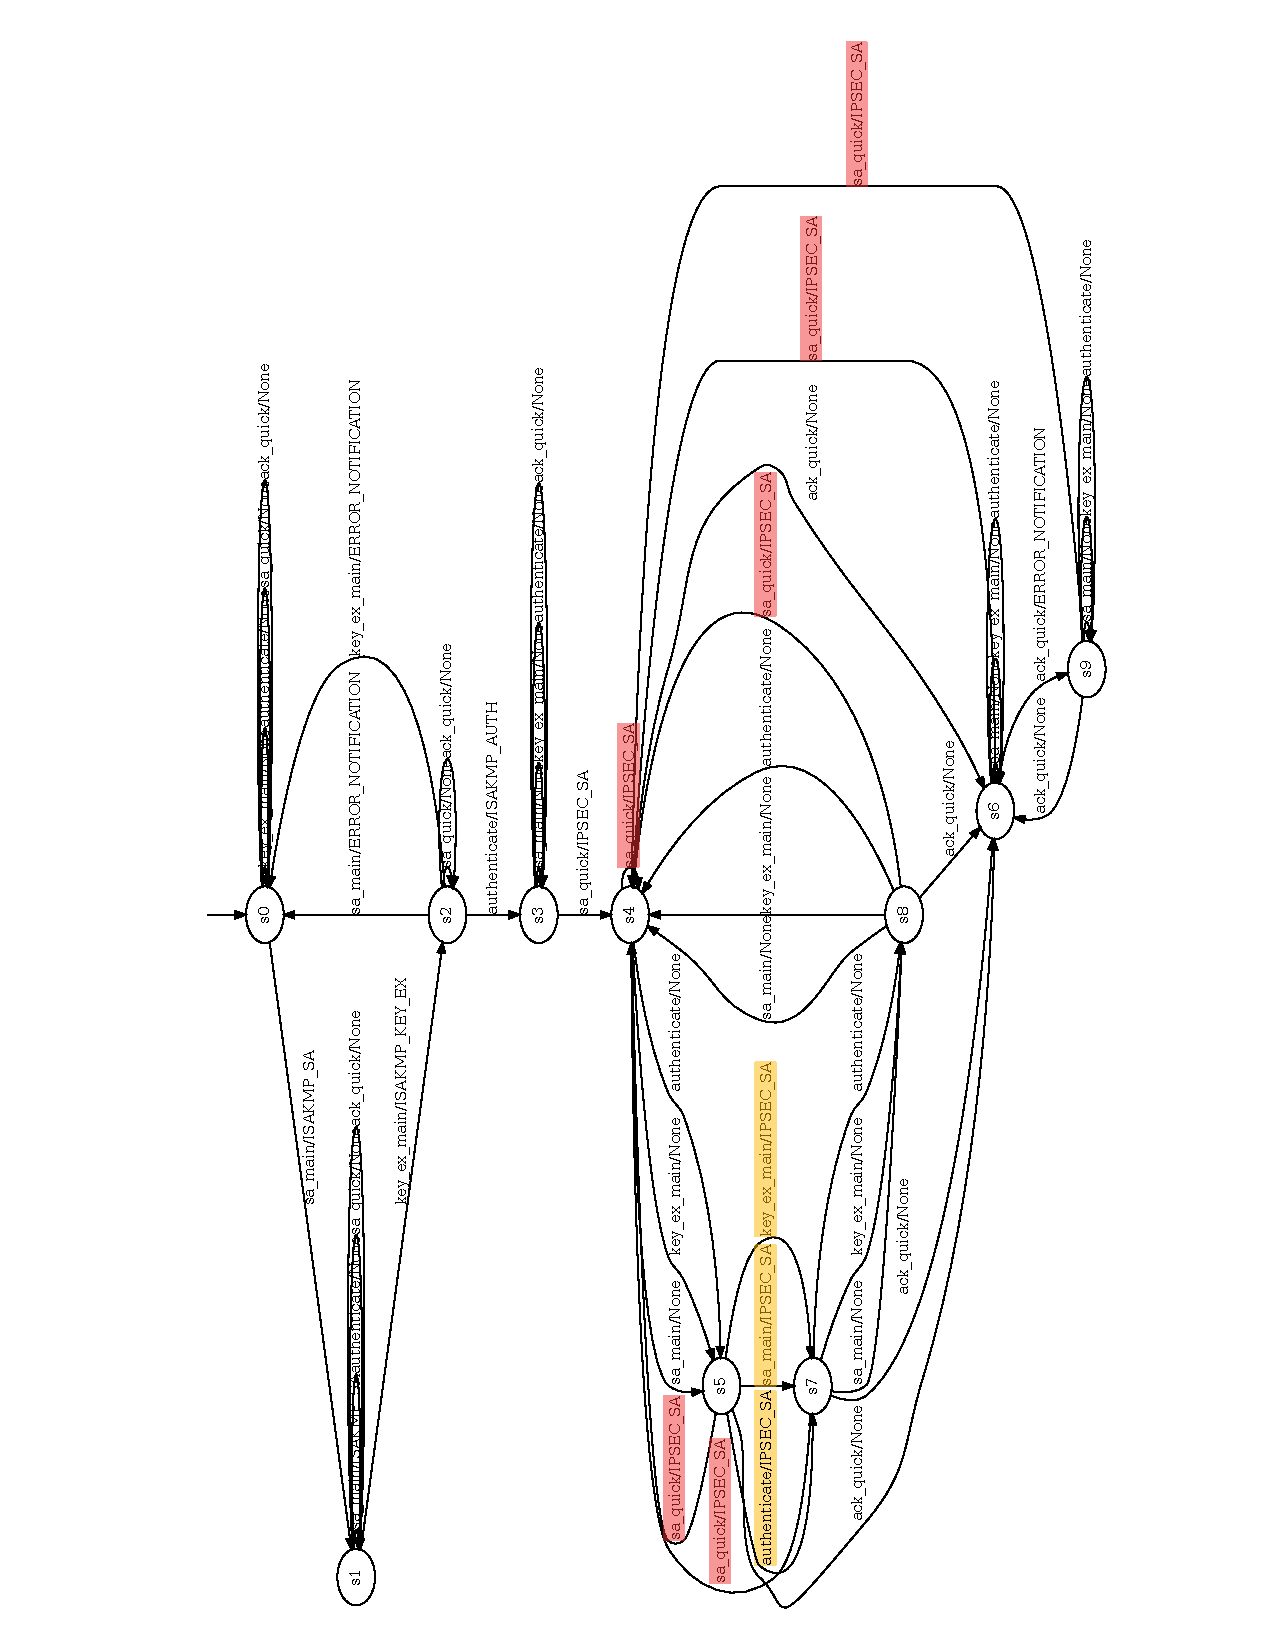
\includegraphics[width=\linewidth, angle=270]{images/models/retransmissions/retrans_case1_lstar}}
	\caption{First commonly learned model of strongSwan server with retransmissions enabled.}
	\label{fig:ret_case1}
	\vspace*{\fill}
\end{figure}

Moving on to an examination of the first common model itself, we can clearly see a separation between the two phases. Phase one completes in state \emph{s3}, and phase two begins right thereafter with the transition from state \emph{s3} to \emph{s4}. While phase one looks very clean and is in fact identical to the model learned with retransmission-filtering enabled, phase two has many unexpected transitions caused by retransmissions. For example, all three transitions from state \emph{s5} to \emph{s7} via \emph{authenticate}, \emph{sa\_main} and \emph{key\_ex\_main}, highlighted in yellow, return a valid \emph{IPSEC SA} response. This should be impossible, as phase one messages are to be ignored while in phase two. However, due to specific timings of retransmissions, our communication interface can occasionally happen to be listening for a server response of a regular phase two communication, when the \ac{sul} sends a retransmission for previous \emph{sa\_quick} message. This causes our framework to treat the received retransmission as the response for the phase two message, when in fact, it is not. We can see multiple incoming and outgoing transitions of state \emph{s4}, highlighted in red, that further exhibit this behavior.
Another noticeable property of the learned automata, is that past state \emph{s2}, no paths lead back to the initial state. This is due to the fact that our input alphabet for this learned model does not include the delete command. Adding \ac{isakmp} delete to the input alphabet creates transitions from every state back to the initial one, but also dramatically increases the runtime and non-deterministic behavior of the \ac{sul}, as even more retransmissions are triggered. While not part of our input alphabet, it could be included in future work.


\subsubsection*{Second Common Model}

The second common model, seen in Figure \ref{fig:ret_case2}, took approximately 75 minutes (4507 seconds) to learn using the $KV$ algorithm. The model took nine rounds to learn, and consists of twelve states. Of those 75 minutes, roughly 53\% were used for state exploration/output queries and the other 47\% (2382 vs 2126 seconds). 215 output queries were performed by the learning algorithm, requiring 2219 steps, whereas 120 conformance tests were performed, requiring 1964 steps. 

In contrast, when learned with the $L^*$ algorithm, model learning took significantly longer, running for 125 minutes (7520 seconds) over five learning rounds. Here, the split between state exploration and conformance checking was again very distinct, with state exploration taking up approximately 71\% of the total runtime and conformance checking only requiring the remaining 29\% (5393 vs 2126 seconds). Again, the time needed for conformance checking remained largely the same between the two algorithms, however the difference in state exploration/output queries is even larger, with $L^*$ taking 522 output queries.

Examining the model, we can again see a clear separation between the two phases. Phase one for this model is identical to the previous one, as no retransmission occur there. Same as in Figure \ref{fig:ret_case1}, no paths past state \emph{s2} lead back to the initial state. Phase two shows retransmission-induced strange behavior in the transitions \emph{s5} to \emph{s7}, as well as \emph{s11} to \emph{s9}. The strange behavior is again linked to retransmissions, causing phase one inputs, such as \emph{sa\_main}, to result in the valid phase two outputs, such as \emph{IPSEC SA}. The states \emph{s7} and \emph{s11} are separated by two states that do not exhibit any strange behavior, apart from having identical inputs and outputs. The main difference to the first common model is, that strange behavior occurs in two pairs of states, highlighted in yellow, and that these pairs are separated by two states that do not appear to receive any retransmissions, highlighted in red. This is likely caused by the \ac{sut} sending repeated retransmissions, in the same frequency, allowing for two states in between. 

\begin{figure}[ht]
	\vspace*{\fill}
	\noindent
	\hspace*{-5.5\oddsidemargin}%
	\makebox[0pt][l]{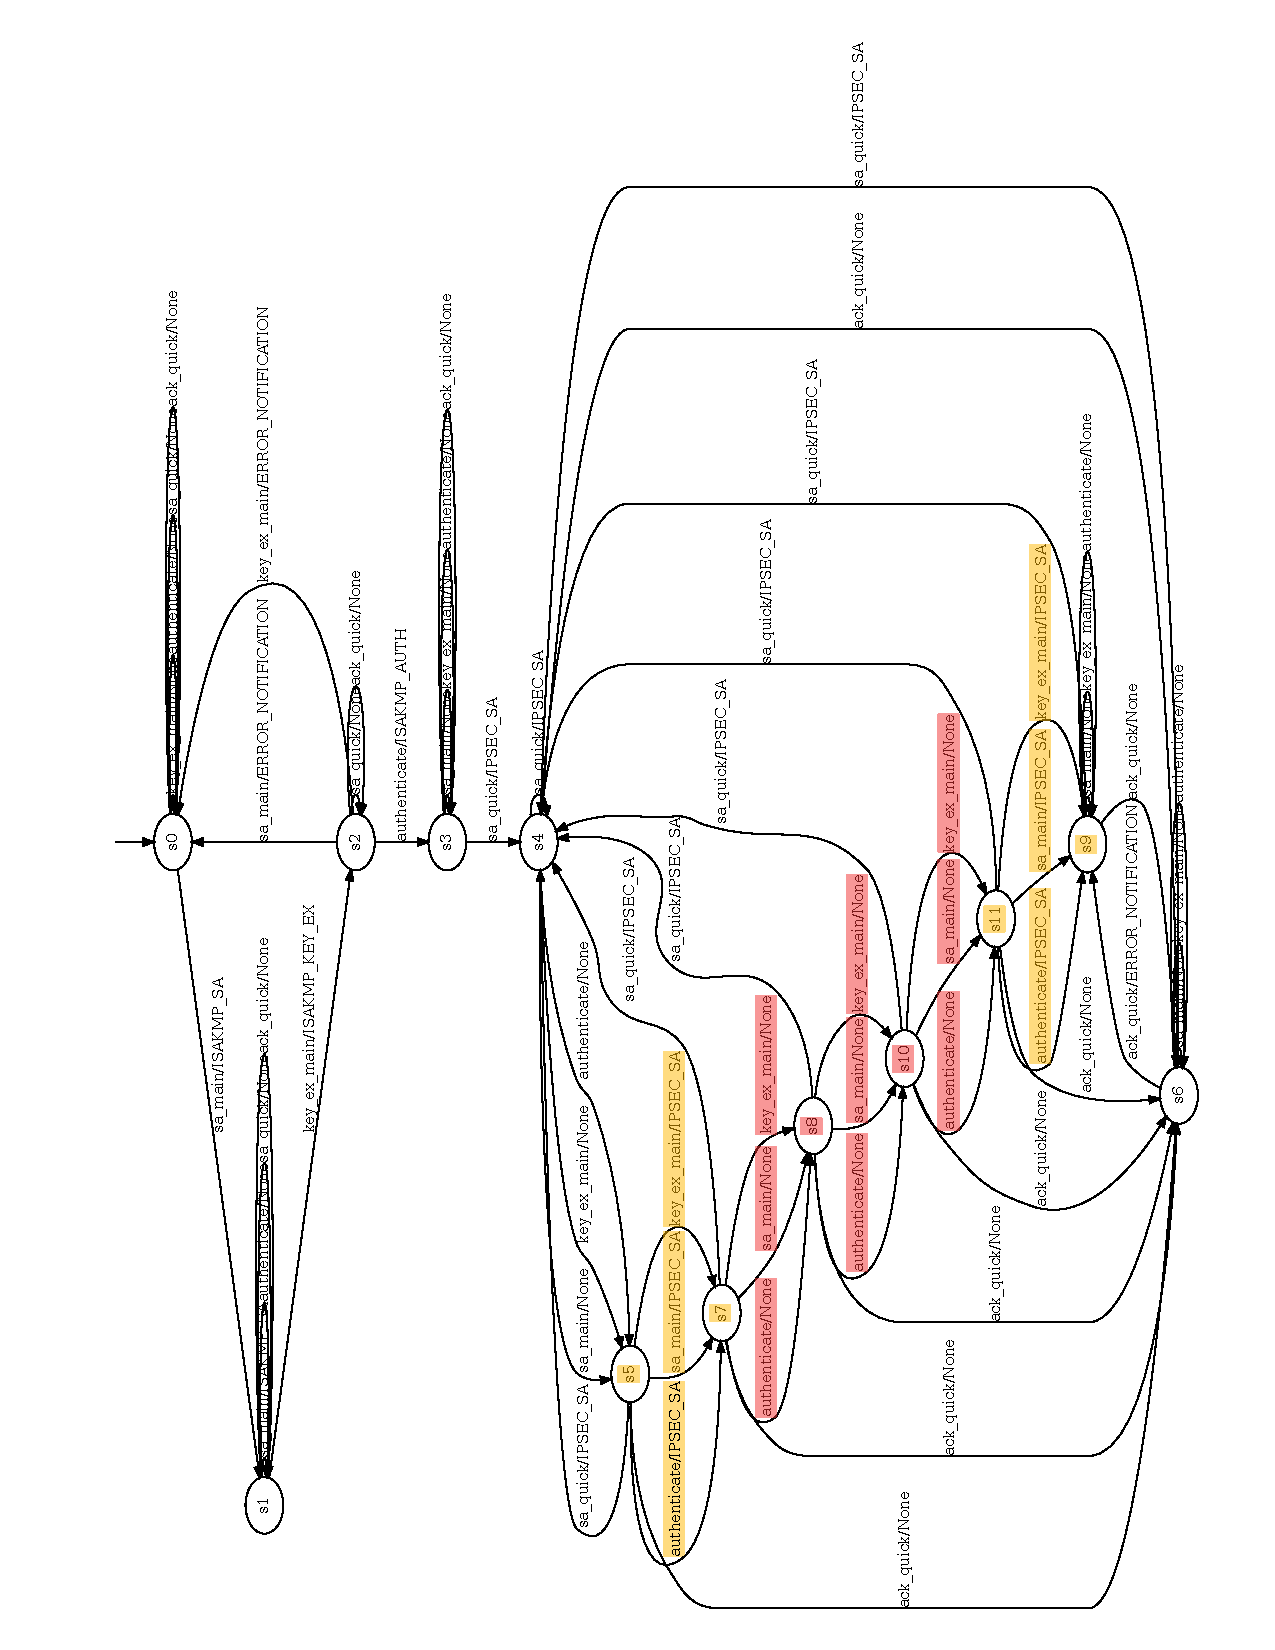
\includegraphics[width=\linewidth, angle=270]{images/models/retransmissions/retrans_case2_lstar}}
	\caption{Second commonly learned strongSwan server model with retransmissions enabled.}
	\label{fig:ret_case2}
	\vspace*{\fill}
\end{figure}
\newpage

\subsubsection*{Clean Base Models}

In comparison, when learning the same server implementation with retransmission-filtering enabled, all non-deterministic behavior vanishes and we get the model shown in Figure~\ref{fig:reference} for every learning attempt. The model has only six states and therefore was learned much more quickly than the previous ones, with learning requiring only approximately 21 minutes (1266 seconds) using the $KV$ algorithm. Learning happened over four rounds, where the time was distributed between state exploration and conformance checking in a 40/60 split (519 vs 747 seconds). This was the only configuration where the conformance checking took longer than state exploration, as highlighted in Table \ref{tab:runtime_summary_kv}. It does however still have the lowest altogether runtime. In comparison, when learned with the $L^*$ algorithm, learning took roughly 36 minutes (2157 seconds), spread over two learning rounds. Of that time, state exploration required roughly 55\% compared to the 45\% needed for conformance checking (1188 vs 969 seconds). Compared to $KV$, state exploration/output queries took more than twice the amount of time to complete.

\begin{table}[h]
	\centering
	\begin{tabular}{|l|l|l|l|l|l|l|}
		\hline
		\rowcolor[HTML]{C0C0C0} 
		Model     		& States & TT (s)  & TL (s)  & TC (s)  & OQ  & CT  \\ \hline
		First Common 	& 10     & 3092 & 1501 & 1591 & 171 & 100 \\ \hline
		Second Common  	& 12     & 4507 & 2382 & 2126 & 215 & 120 \\ \hline
		Base      		& 6      & 1214 & 480  & 734  & 78  & 60  \\ \hline
		Reference 		& 6      & 1447 & 879  & 568  & 174 & 60  \\ \hline
	\end{tabular}
	\caption{KV Runtimes of all the learned strongSwan models.}
	\label{tab:runtime_summary_kv}
\end{table}

Looking at the resulting model more closely, the first four states are again identical to the previous model. This is due to the fact that the retransmissions are only triggered for phase two messages and since they are our only source of non-determinism, there are no differences here. However, the phase two states look wildly different, showing a streamlined behavior that fits our reference \ac{ike} exchange (see Figure \ref{fig:IKEv1}) almost perfectly. The only small difference lies in the additional state \emph{s5} which loops back to state \emph{s4} with an \emph{IPSEC SA} or \emph{ACK} message. This behavior shows how multiple \ac{ipsec} \acp{sa}, each created from a single IKE SA channel, can be used interchangeably for different traffic flows but not simultaneously. As soon as a new \ac{ipsec} \ac{sa} has been established, another \emph{ACK} message can be sent, to finalize the creation of the new \ac{ipsec} \ac{sa}. In other words, the extra state is there to show that a single \ac{ipsec} \ac{sa} cannot be acknowledged twice, and instead a new \ac{sa} must be created first. 

\begin{figure}[ht]
	\vspace*{\fill}
	\noindent
	\hspace*{-5.5\oddsidemargin}%
	\makebox[0pt][l]{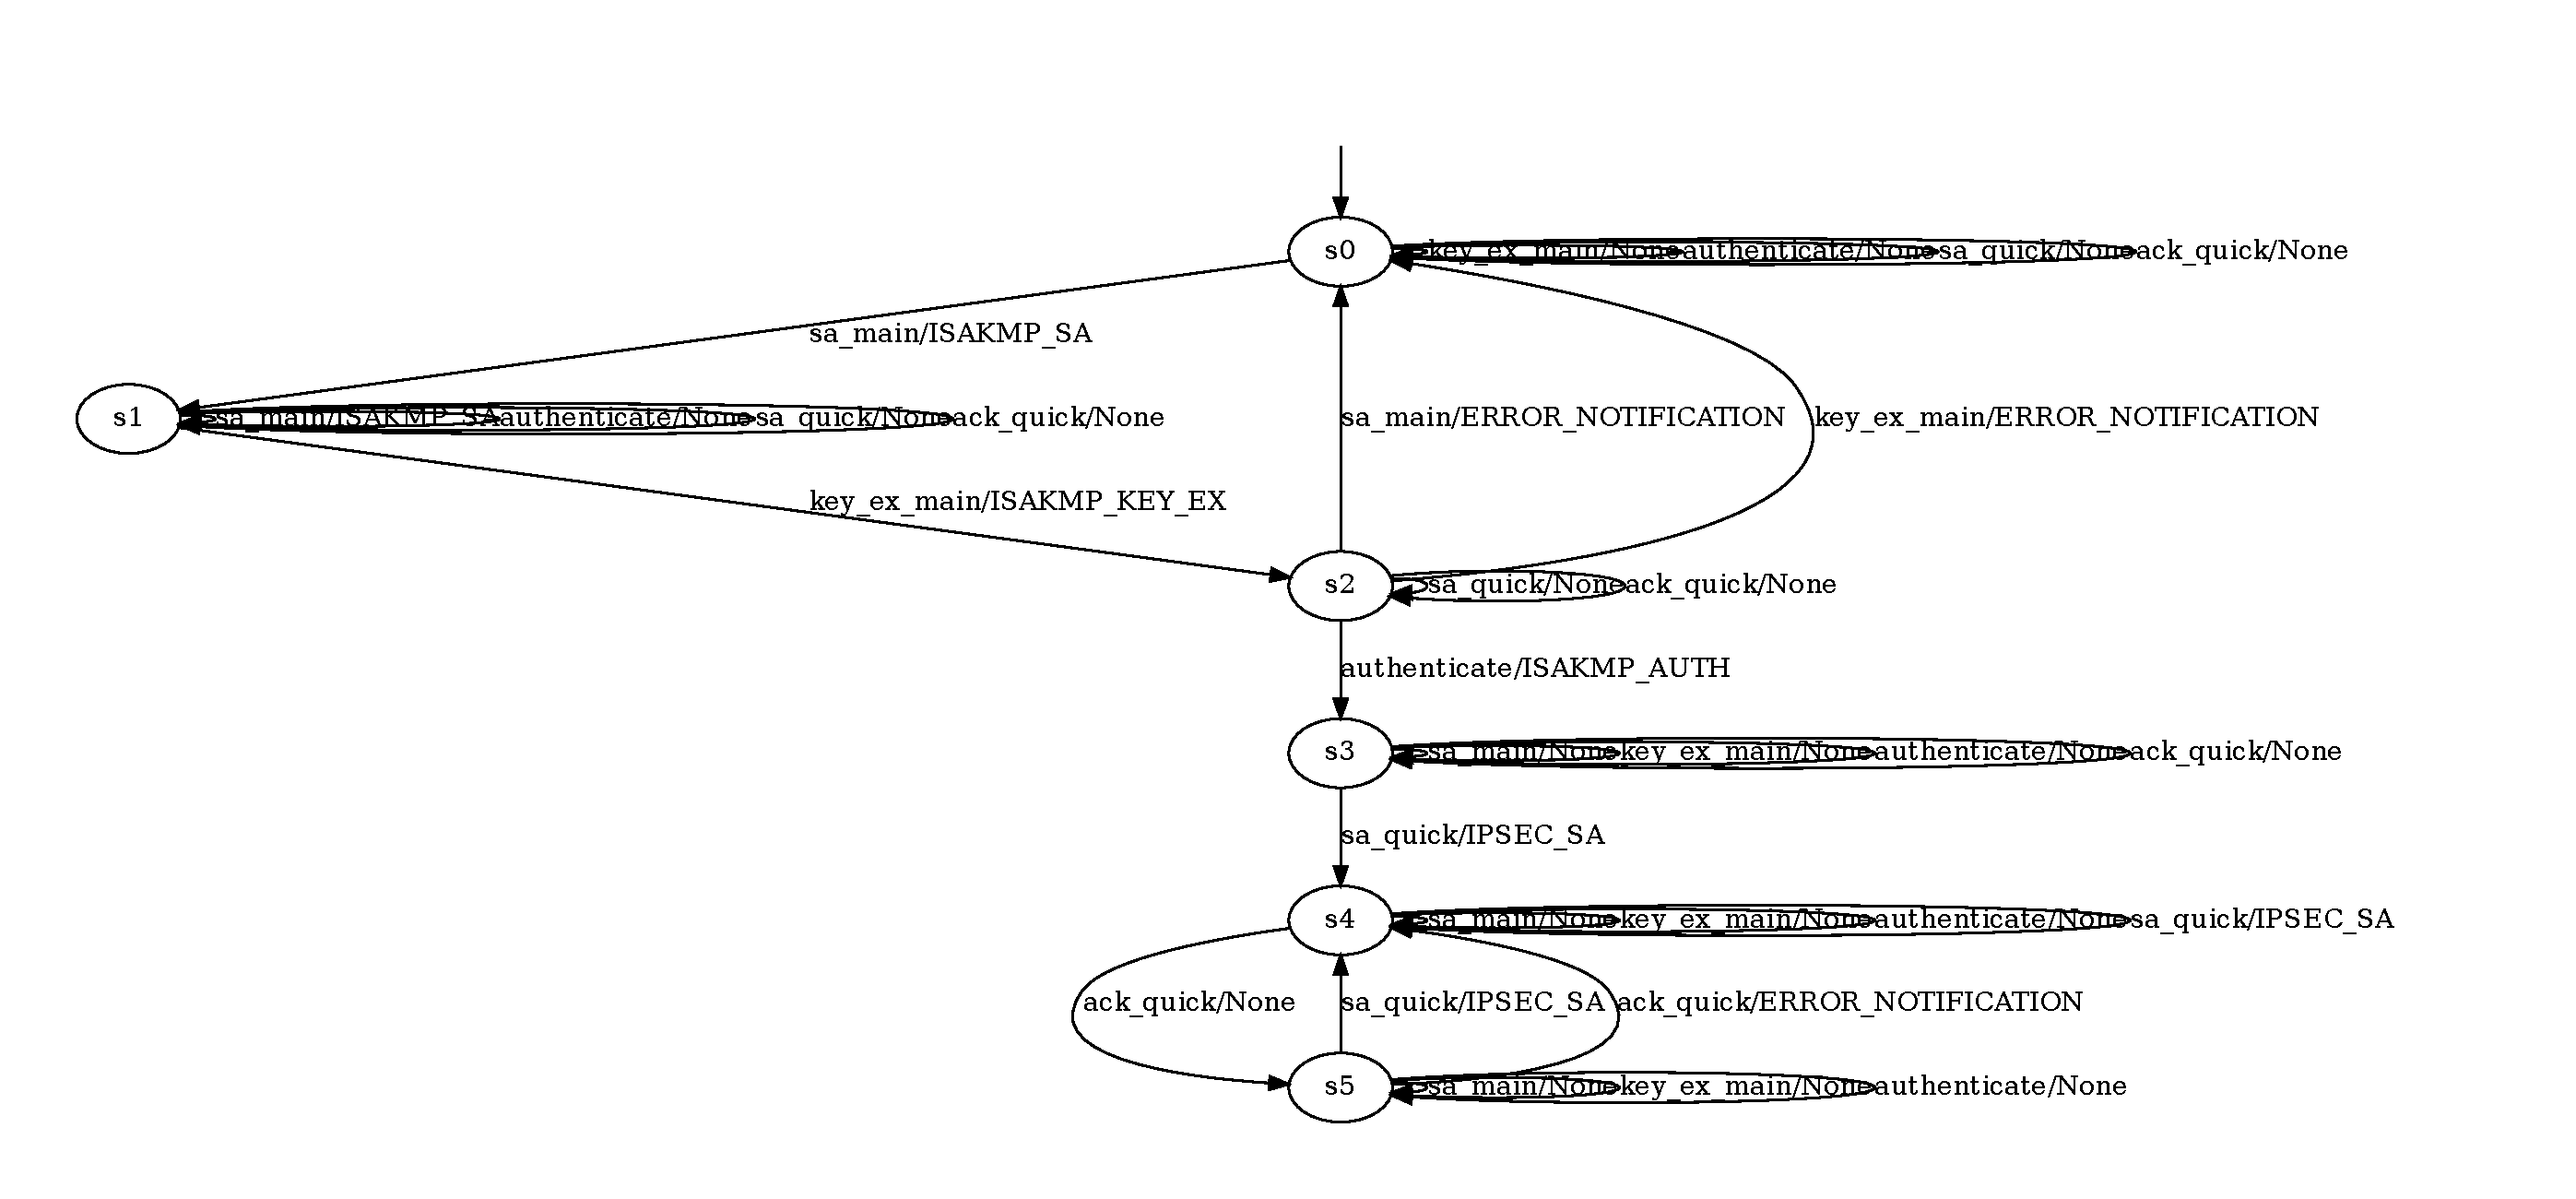
\includegraphics[width=1.4\linewidth]{images/models/Reference}}
	\caption{Clean strongSwan model learned using retransmission-filtering.}
	\label{fig:reference}
	\vspace*{\fill}
\end{figure}

\subsubsection*{Fuzzing Reference Models}
% Error model
Figure \ref{fig:withfilterwitherrors} shows the (simplified, with self-transitions removed for readability) reference model used for fuzzing the strongSwan server, learned with retransmission-filtering enabled. The DOT file of the full model is provided in Appendix~\ref{app::dot}. Additionally, the input alphabet was expanded to include an additional erroneous version of each input that maps to an erroneous input. Thanks to the retransmission-filtering, the same model could be learned every time. Using the $KV$ algorithm, it took roughly 24 minutes (1447 seconds) to learn. The model took between five and four learning rounds to learn and consists of six states. Roughly 60\% of the total learning time was spent on state exploration/output queries and the remaining 40\% on conformance checking (879 vs 568 seconds). Alternatively, when learned using the $L^*$ algorithm, the model took a total of 51 minutes (3078 seconds) to learn over a single learning round. The 51 minutes were split between state exploration and conformance checking in a 80/20 split (2500 vs 578 seconds), with state exploration requiring 600 output queries. Interesting to note is the large difference in conformance checking runtime between the two algorithms. For learning the reference model using $L^*$, state exploration takes up more than 80\% of the total runtime, which is the highest percentage for all the learned models, as can been seen highlighted in the runtime summary in Table \ref{tab:runtime_summary_lstar}.

\begin{table}[h]
	\centering
	\begin{tabular}{|l|l|l|l|l|l|l|}
		\hline
		\rowcolor[HTML]{C0C0C0} 
		Model     & States & TT (s)   & TL (s)   & TC (s)   & OQ  & CT  \\ \hline
		First Common  & 10     & 5094 & 3489 & 1605 & 462 & 100 \\ \hline
		Second Common  & 12     & 7520 & 5393 & 2126 & 522 & 120 \\ \hline
		Base      & 6      & 1652 & 899  & 753  & 177 & 60  \\ \hline
		Fuzzing Ref. & 6      & 3078 & 2500 & 578  & 600 & 60  \\ \hline
	\end{tabular}
	\caption{$L^*$ Runtimes of all the learned strongSwan models.}
	\label{tab:runtime_summary_lstar}
\end{table}

The model looks largely identical to the previous model, apart from some additional self and error transitions (self transitions not shown here in the simplified version). Notably, there is an error transition from state \emph{s4} to \emph{s5}, via \emph{sa\_quick\_err}. This error transition implies, that a valid \ac{ipsec} \ac{sa} is required for \emph{ack\_quick} to work. In other words, the erroneous \ac{sa} is insufficient for the server to accept an ensuing acknowledgment. If attempted, the strongSwan server returns an error message. For the same reason there is another error transition from state \emph{s3} to \emph{s5}, highlighting that one cannot complete the \ac{ipsec} handshake with invalid \ac{ipsec} \ac{sa} packets. In summation, the mentioned error transitions simply show that a valid \ac{ipsec} \ac{sa} must be created before it can be acknowledged. Note, that the DOT files of all models can be found in Appendix~\ref{app::dot} and larger PDF files of all models are available as supplementary material\footnote{\url{https://github.com/benjowun/VPN-AL}}.

\begin{figure}
	\centering
	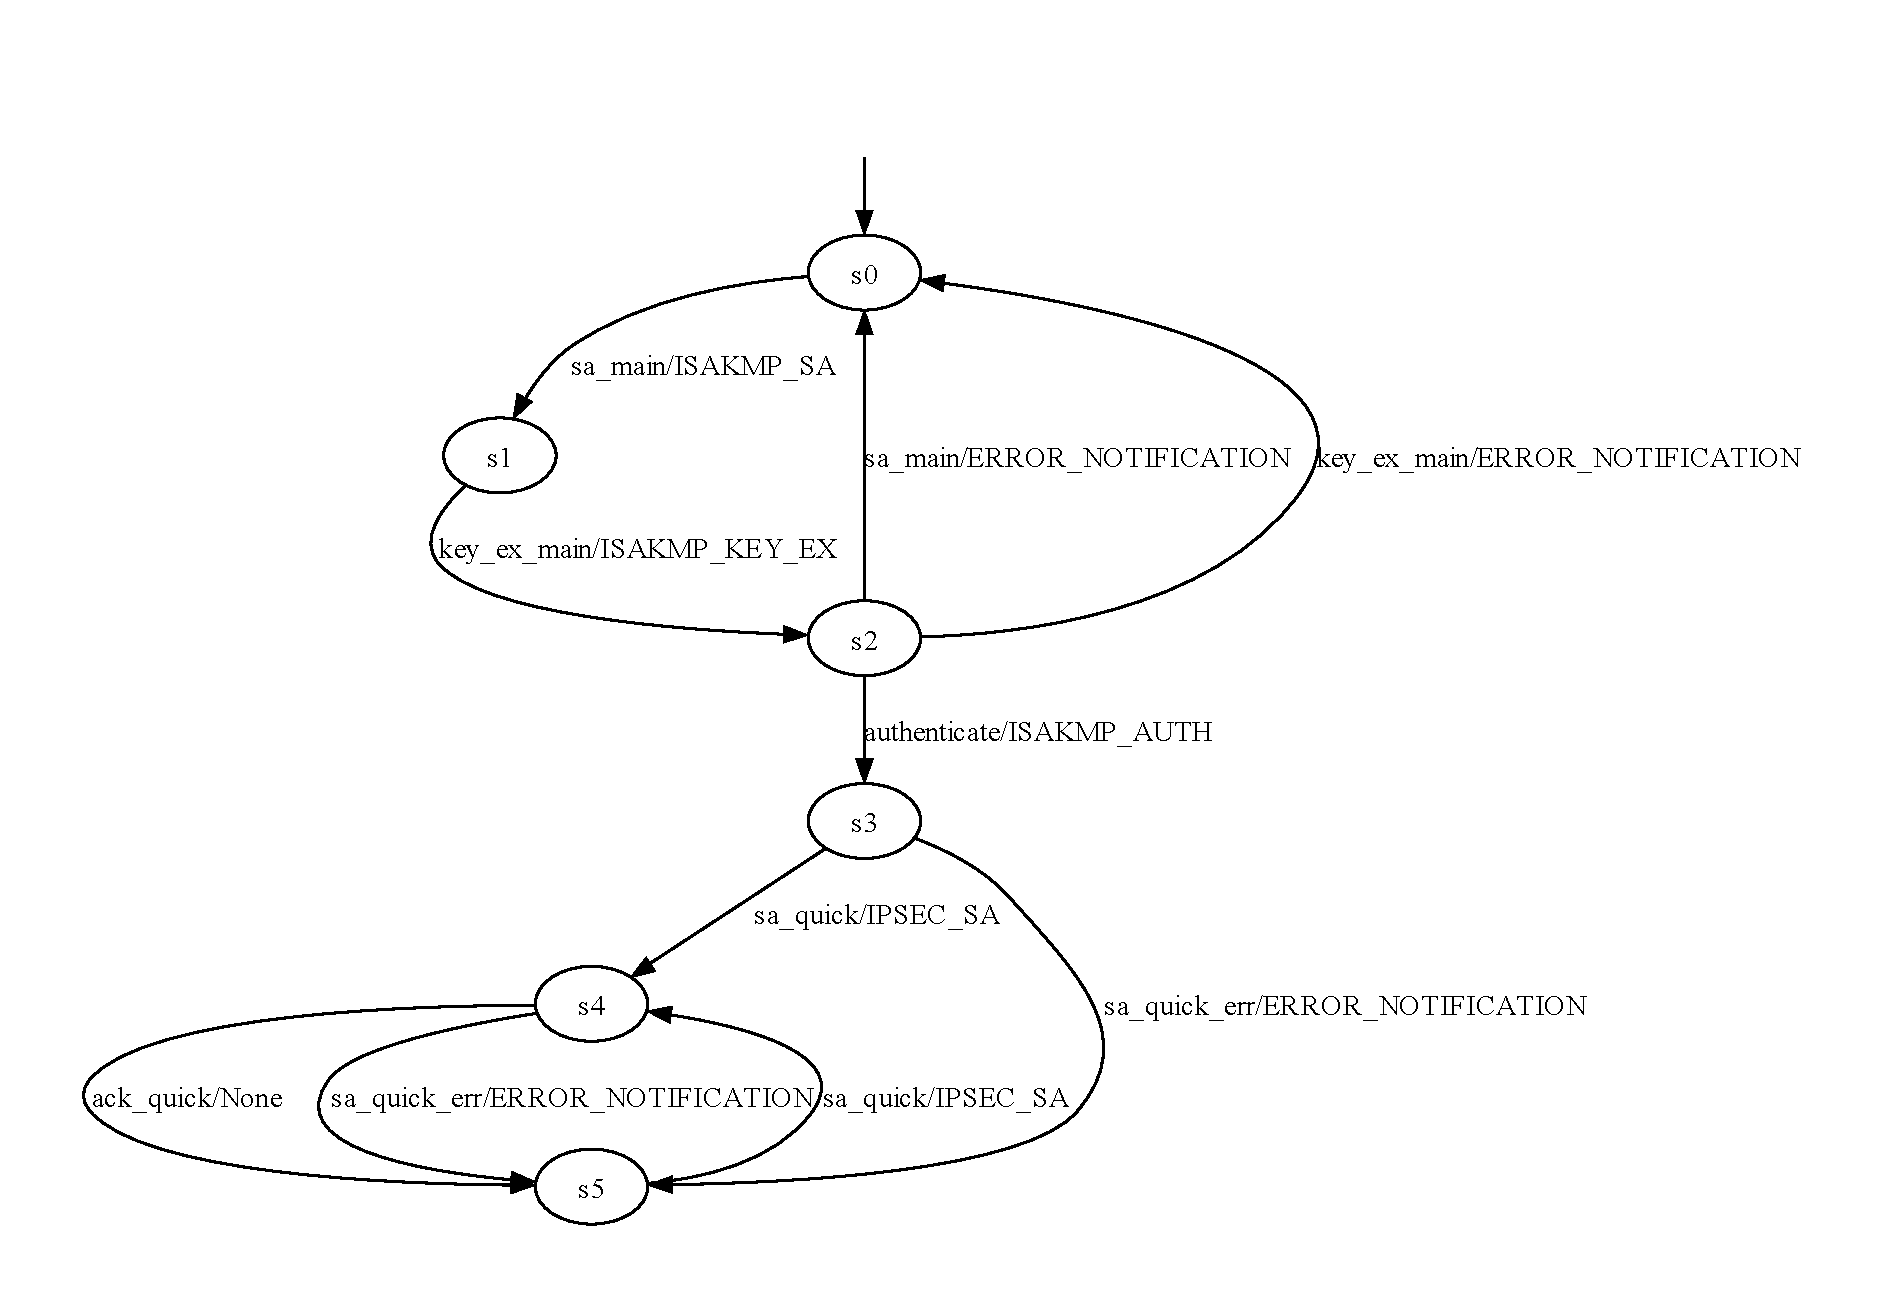
\includegraphics[width=\linewidth]{images/models/strongSwanErrKV}
	\caption{(Simplified) strongSwan model with malformed messages in the input alphabet.}
	\label{fig:withfilterwitherrors}
\end{figure}


Table~\ref{tab:runtime_summary_averages} shows the average statistics of both learning algorithms over all four learned strongSwan models (averages of $L^*$ and $KV$ combined in one cell). As expected, models consisting of more states took longer to learn than those with less. For the two models with an identical amount of states, namely the Base and Fuzzing Reference models, the combined number of queries sent is a more suited indicator for the expected runtime. In general, the combined number of queries serves as a good indicator for how long each model will take to learn. 

\begin{table}[h]
	\centering
	\begin{tabular}{|l|l|l|l|l|l|l|}
		\hline
		\rowcolor[HTML]{C0C0C0} 
		Model    	& States & TT (s)   & TL (s)   	  & TC (s)   & OQ  & CT  \\ \hline
		Common A  	& 10     & 4048 	  & 2495	 	  & 1553 	 & 317 & 100 \\ \hline
		Common B  	& 12     & 6014 	  & 3888		  & 2126 	 & 369 & 120 \\ \hline
		Base      	& 6      & 1433 	  & 690 		  & 744  	 & 128 & 60  \\ \hline
		Fuzzing Ref.& 6      & 2263 	  & 1690		  & 573  	 & 387 & 60  \\ \hline
	\end{tabular}
	\caption{Runtimes averages of both learning algorithms of all the learned strongSwan models.}
	\label{tab:runtime_summary_averages}
\end{table}

\subsection{Learned libreswan Models}
Figure \ref{fig:learnedmodellibresimple} shows the libreswan clean base model, learned using the same input alphabet and retransmission-filtering rules. The corresponding strongSwan model is the strongSwan Base model, shown in Figure~\ref{fig:reference}. The model is very simple, consisting of only four states. Learning occurred over two rounds using the $KV$, and only one round, using the $L^*$ algorithm. Despite the aforementioned reset workaround potentially affecting runtimes and therefore them being excluded from statistics, some runtime-agnostic metrics, such as the number of required queries and steps, are still provided. Using the $KV$ algorithm, 36 output queries and 321 steps were required by the learning algorithm. Conversely, $L^*$ required 100 output queries and 350 input steps. Both algorithms required 40 conformance tests for equivalence checking, with the $KV$ algorithm however requiring roughly 660 steps, compared to the 460 of the $L^*$ algorithm. With respect to runtime, $KV$ did outperform $L^*$, but it is important to again note, that any runtime measurements for libreswan are unreliable and cannot be compared with the strongSwan runtimes, due to the reset workaround.

The learned libreswan base model itself is noticeably smaller than its strongSwan equivalent, having two less states. In addition, the libreswan model is very linear, with each state being forced to occur subsequently. This is due to how libreswan handles errors and invalid messages, completely ignoring most error types that would lead to connection resets with strongSwan. This behavior is also what forced us to implement a workaround for the reset functionality, as error messages do not cause the libreswan phase one \ac{isakmp} connection to be closed. Another key difference is that following the initial key exchange in phase one, the libreswan server does return error messages when presented with another unencrypted key exchange request, but does not close the affected connection. In contrast, strongSwan simply ignores them in phase two resulting in a None response in the model. However, if an additional key exchange request is sent to a strongSwan server before phase one is completed, the server returns an error and aborts the connection. The key difference here being the closing of the connection on error, which again explains the more complicated strongSwan model, compared to the linear libreswan one. This difference can, e.g., be seen when comparing the transition of Figure~\ref{fig:reference}, state \emph{s2} to \emph{s0}, with state \emph{s3} of Figure~\ref{fig:learnedmodellibresimple}, noting the lack of a transition back to the initial state for the libreswan model. Finally, there is a distinct lack of error messages for not-yet established \ac{ipsec} SA acknowledgments on the libreswan server, resulting in both \emph{sa\_quick} and \emph{ack\_quick} remaining in the same state. 

In summation, one can say that the strongSwan server is stricter with their error handling, closing connections if errors are encountered, whereas libreswan is more error-tolerant, preferring to keep connections regardless. These implementation details are clearly visible in the presented models, with the libreswan model being considerably more simple.

\begin{figure}
	\centering
	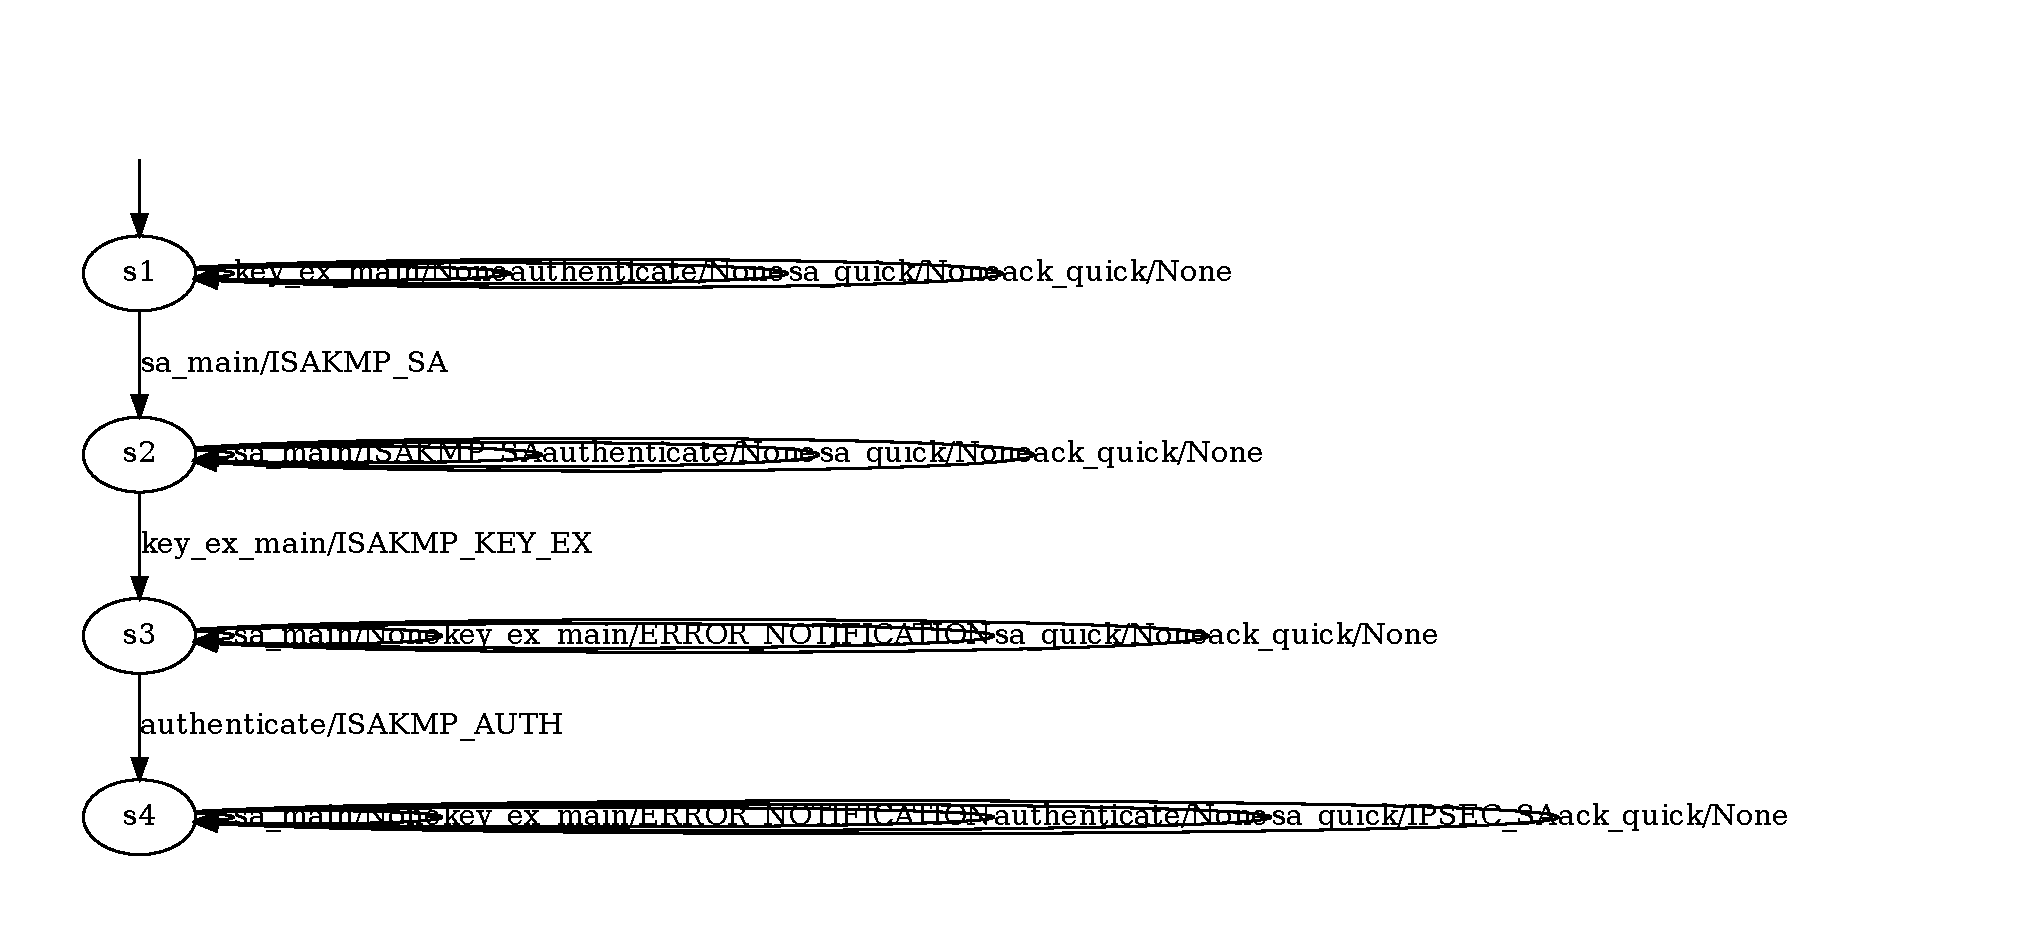
\includegraphics[width=\linewidth]{images/models/LearnedModelLibreSimple}
	\caption{Clean libreswan model learned using retransmission-filtering.}
	\label{fig:learnedmodellibresimple}
\end{figure}

The libreswan version of the fuzzing reference model is again simpler than its strongSwan counterpart, consisting of one less state (five vs six) than the strongSwan fuzzing reference model. The DOT file of the full automata can be found in Appendix~\ref{app::dot}. Figure~\ref{fig:learnedmodellibrereference} shows a strongly simplified model, without self-transitions, highlighting the new state \emph{s2}. It looks largely identical to the libreswan base model, with the notable addition of a left branch in the model (state \emph{s1} to \emph{s2}), where an erroneous \emph{sa\_main\_err} packet is sent at the start of the connection. This causes the server to become impossible to establish a connection with (with our setup), as libreswan ignores any further attempts with the same initiator cookie, following an invalid one, regardless of their correctness. The server does not leave this error state any more, as due to the \emph{uniqids} setting mentioned in Chapter~\ref{chap:Setup}, all following \emph{ISAKMP\_SA} packets will use the same ID. While the admittedly a rather uncommon server setup (primarily used here due to simplify our mapper class), it could be considered a design flaw, to block valid \emph{ISAKMP\_SA} packets from replacing a broken connection when using the \emph{uniqids} setting, as this renders the connection unusable. A valid use-case for this setting could be wanting to connect multiple users using a single \ac{ike} connection.

As switching to a randomly generated initiator cookies system would have negatively affected the strongSwan setup, the decision was made against a random-initiator cookie redesign. Especially since the libreswan setup already required a workaround for its reset method, potentially skewing results, the additional reworks were considered not worth the effort, but should be considered for future work.

\begin{figure}
	\centering
	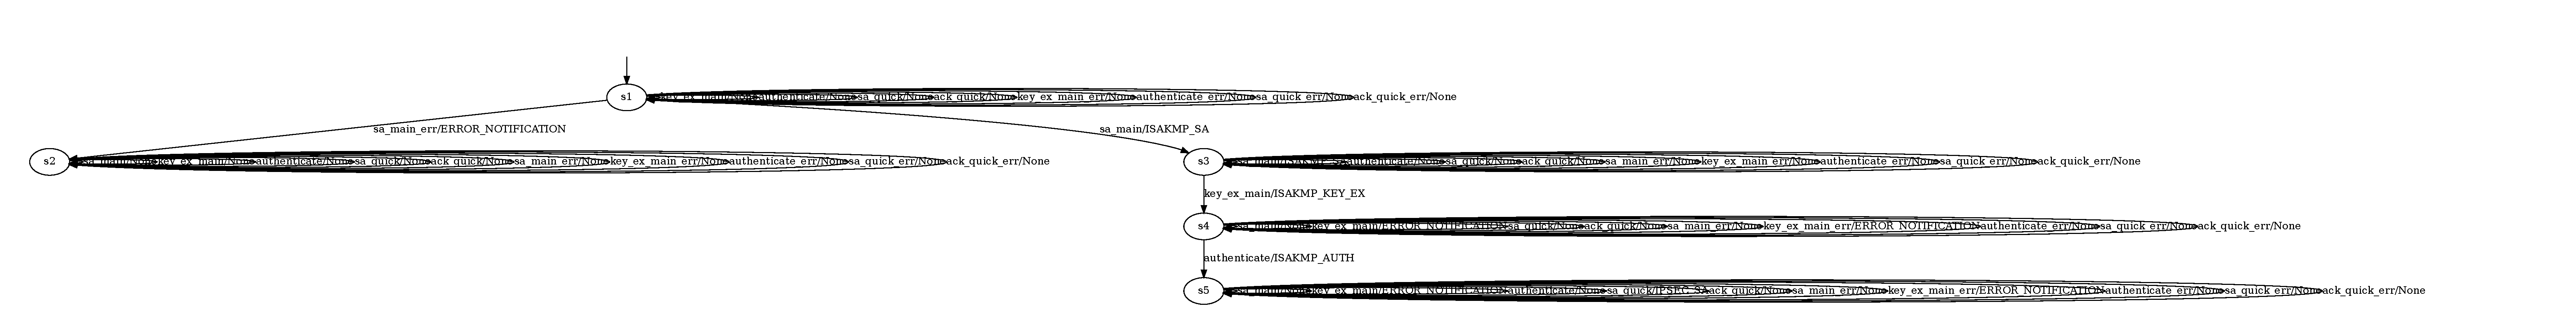
\includegraphics[width=0.7\linewidth]{images/models/LearnedModelLibreReference}
	\caption{(Simplified) libreswan model with malformed messages in the input alphabet.}
	\label{fig:learnedmodellibrereference}
\end{figure}

\subsection{Comparing $KV$ and $L^*$} \label{subsec:comp_kv_lstar}
% section copmaring KV and Lstar
Table \ref{tab:compkvlstar} shows average performance statistics over 20 learning attempts for both learning algorithms on the strongSwan server. The models were learned with retransmission-filtering enabled. The same hardware and software configurations were used as described in Chapter~\ref{chap:Setup} with the learning program set up on a VirtualBox 6.1 \ac{vm} allotted 4GB of memory and one CPU core. We used all the basic packets for our input alphabet, so
\emph{sa\_main}, \emph{key\_ex\_main}, \emph{authenticate}, \emph{sa\_quick} and \emph{ack\_quick}. The model learned is the clean model seen in Figure \ref{fig:reference}. Table~\ref{tab:compkvlstar} shows the metric on the left and the respective averages for the $L^*$ and $KV$ learning algorithms respectively on the right. Interesting results are highlighted in bold. From top to bottom, the metrics measured are as follows. Learning rounds refers to the number of rounds the learning algorithms had to run for, or in other words, how many hypotheses they needed to propose to the teacher in order to correctly learn the \ac{sul}. Total time is the total time needed by the algorithm from start to the finished model. The total time can be split into time spent on the state exploration and time spent on equivalence queries. Learning output queries refers to the number of output queries sent to the SUL while learning steps to the number of individual inputs executed on the \ac{sut}. Analogously, equivalence oracle queries refers to the equivalence queries sent to the SUL and equivalence oracle steps to the inputs executed by the equivalence oracle. Finally, output queries saved by caching details the performance boost gained by caching output queries, with the value indicating the number of queries saved.

As the only difference between the two configurations tested was the choice of learning algorithm, intuitively one expects relevant fields to vary the most with equivalence oracle field to be largely unchanged. This intuition is confirmed by our experiments, wherein while the time spent on equivalence queries was very similar, with both requiring the same number of equivalence oracle queries for conformance checking. In contrast, the time spent on output queries differs greatly between the two model-learning algorithms. The $L^*$ algorithm required almost double the number of output queries than its $KV$ counterpart. As communication with the \ac{sut} is the main performance bottleneck and output queries make up a large portion of this communication, this change naturally led to a significantly better runtime for $KV$, with total time spent on the learning algorithm being close to half that of the $L^*$ algorithm. This difference in time spent on the learning algorithm meant, that for this experiment, the $KV$ algorithm learned a model in roughly 75\% of the time needed by the $L^*$ algorithm. Looking only at the learning algorithm, $KV$ performed roughly twice as well as its counterpart. As the same equivalence checking algorithm was used for both attempts, the identical number of equivalence oracle queries makes sense. Another noticeable difference can be observed in the number of output queries saved by caching. Here, $KV$ saves more than double the amount $L^*$ does, indicating a better caching implementation. In summation, we found the $KV$ algorithm to be better suited for our learning setup and solely used it for fuzzing. 

Little variance was observed throughout all learning attempts so the sample size of 20 learning attempts each is believed to be representative. However, for even more accurate results the experiment should be carried out again for even more input sequences. Additionally, it might be interesting to compare the performance of various equivalence oracles for this learning setup.

\begin{table}[h]
	\centering
	\begin{tabular}{ |p{6.5cm}||p{1cm}|p{1cm}|  }
		\hline
		\multicolumn{3}{|c|}{\textbf{Learning Algorithm Performance (Averages)}} \\
		\hline
		\textbf{Metric} & $\mathbf{L^*}$ & $\mathbf{KV}$ \\
		\hline
		Learning Rounds							&	2				&	4 				\\
		Total Time (s)							&   1652			& 	1214   			\\
		Time Learning Algorithm	(s)				&	\textbf{899}	& 	\textbf{480}	\\
		Time Equivalence Checks (s)				& 	753				& 	734			\\
		Learning Output Queries 				&   \textbf{177}	& 	\textbf{78}		\\
		Learning Steps							& 	856	  			& 	676   			\\
		Equivalence Oracle Queries				& 	60  			&  	60				\\
		Equivalence Oracle Steps				& 	747  			&  	934				\\
		Output Queries Saved by Caching			& 	\textbf{13}		&  	\textbf{30}				\\
		\hline
	\end{tabular}
	\caption{Comparison of the $L^*$ and $KV$ learning algorithms.}
	\label{tab:compkvlstar}
\end{table}
\newpage

\subsection{Library Error} \label{subsec:liberror}
% section with discovered bug
Another notable finding from the model learning phase, which demonstrates the usefulness of \ac{aal} from a testing standpoint, was the discovery of a bug in a used Python Diffie-Hellman key exchange library. The bug was only found thanks to the exhaustive number of packets sent with our mapper class and due to the non-determinism checks implemented in \textsc{AALpy}. Despite our best efforts in removing the non-deterministic behavior from our learning process, we would still get occasional non-determinism errors at random points while learning. This problem persisted over several weeks due to the fact that the errors occurred randomly and only sporadically during some learning attempts. Initially we believed this to be also caused by retransmissions, but since the problems persisted even after introducing retransmission-filtering, that possibility was ruled out. The other option was of course problems in our implementation of the \ac{ipsec} protocol. Therefore, a lot of time was invested into painstakingly comparing logs and packet captures between our implementation and the \ac{sul} to ensure that everything lined up, since \textsc{AALpy} was still reporting non-determinism errors. Finally, a small discrepancy between the two logs was discovered and through it, that the problems were not in fact caused by our implementation, but by a used Python library. It turns out there was a very niche bug in a used Diffie-Hellman Python library~\cite{topdappdh}, where if the \ac{msb} was a zero, it would be omitted from the response, causing the local result to be one byte shorter than the value calculated by the \ac{sul}. As this would only occur in the rare case where the \ac{msb} of the DH exchange was zero, this explains the random and difficult to reproduce nature of the bug. This behavior was undocumented and happened in a function call that allowed specifying the length of the returned key. As the library is not a very widespread one, the impact of this bug is presumably not very high. Regardless, it could compromise the security of affected systems and therefore the maintainer of the library has been notified of the problem. Due to the elusive nature of this bug, it would very likely not have been noticed without the exhaustive communication done by the model-learning process and without seeing the slight differences in the resulting models that did not crash during the learning process.

\section{Fuzzing Results} \label{sec:fuzzresults}
We used model-based fuzzing to test the two \ac{ipsec} \ac{ike}v1 \acp{sut}. Our fuzzer supports testing inputs in the context of input sequences, to ensure an identical state on the \ac{sut} for each fuzzed input. To that end, we developed a custom fuzzer supporting multiple methods of generating the input sequences to be tested, filtering, search and genetic algorithm-based input-sequence generation, as described in Chapter~\ref{chap:Fuzzing}. All fuzzing took place in the same isolated network described in Chapter~\ref{chap:Setup}. The used fuzzing reference models can be seen above in figures \ref{fig:reference} and \ref{fig:learnedmodellibrereference}, for strongSwan and libreswan respectively. This section presents the results of using our custom fuzzer to fuzz both a strongSwan, as well as a libreswan \ac{ipsec} server. Different input-sequence generation methods were used and contrasted, comparing performance and discovered findings. Most methods found the same issues, however the search-based input-sequence generation method proved to be the fastest and the genetic method resulted in the best fitness score. Randomly generated input sequences serving as a baseline did not discover all the findings. 

\subsection{Findings} \label{subsec:findings}
Our fuzzer was very successful in discovering new behavior not covered by the reference model, finding new cases for almost every input sequence tested with both input-sequence generation methods. As discovered new behavior does not necessarily indicate that the new behavior is harmful, the discovered new transitions still had to be manually parsed for particularly interesting behavior. By analyzing the specific concrete inputs leading to new transitions, we discovered two undocumented instances of the \ac{sut} not following RFC specifications. Unfortunately, a lot of ``non-findings'' were discovered as well, with non-findings referring to new behavior not covered by the reference model, but also not exhibiting undocumented or otherwise interesting behavior. Some of these non-findings could be removed by simply specifying some fields which should not be fuzzed. Unfortunately, this approach requires manually going through and verifying that none of the discovered behavior is interesting. Alternatively, it might be possible to use the discovered new behavior to generate a suite of tests checking for common exploitable vulnerabilities, such as buffer overflows and memory leaks. However, this goes beyond the scope of this thesis.

To further reduce the amount of information that had to be manually reviewed, we improved the fuzzer by temporarily adding newly learned states and transitions to the reference model as soon as they are discovered. This stops the fuzzer from repeatedly discovering the same new behavior with different variations of the same fuzzed input, leading to far less manual reviewing being required. For completeness sake, we first present some of the more interesting or common non-findings, followed by the two discovered deviations from the RFC specifications. Unless otherwise mentioned, all findings were found on both tested \ac{ipsec} servers.

An example of a non-finding that is typically categorized as noise is the discovery of new behavior by changing the initiator/responder cookies as part of fuzzing. These cookies are used in part to identify the members of a \ac{vpn} connection. The new behavior was detected, as during the learning of the reference model, the cookies were not changed mid-input sequence execution, as this causes the \ac{sut} to think it is communicating with a different user and if it doesn't know that user, to simply discard the message. As fuzzing the cookie fields did not lead to any errors on the server side and greatly complicated the mapper class, this field was removed from the fuzzing scope. 

Another non-finding was discovered while fuzzing the field indicating the number of proposals in the \emph{ISAKMP SA} packet. While testing various randomly chosen lengths, every time the length was set to one, the fuzzer indicated, that a new state had been found. This behavior was caused due to our implementation of both the fuzzer and base reference model. Our \emph{ISAKMP SA} packet always contains exactly one proposal and the packet being fuzzed is assumed to be incorrect. However, in this case, the field is, by fuzzing through random numbers, every so often set to a valid value (namely one), resulting in a mismatch between the expected (error) and actual (normal) response. 
Yet another cause of many non-findings during fuzzing were the various packets containing hashes, e.g., \emph{ACK} and \emph{AUTH}. Fuzzing these hashes proved to be problematic, as random changes to the hashes causes the server response encryption to no longer match the mapper class, making decryption impossible. Therefore, errors had to be manually examined in the strongSwan logs. Seeing as no crashes or other unexpected errors were observed, fuzzing hashes was reduced in the overall fuzzer. 

Overall, while examining and testing the discovered new behavior helped improve our overall understanding of the \ac{ipsec} protocol, it rarely resulted in the discovery of any actual undefined/undocumented behavior. However, in two separate cases, actual deviations from the relevant RFC specifications were observed with the \acp{sut}. 

The first of these deviations was discovered while fuzzing the \ac{isakmp} header length field. This field is specified by RFC 2409~\cite{rfc:isakmp} (\ac{isakmp} protocol definition), as the length of the entire \ac{isakmp} packet. When manually going through the results of the fuzzer, a significant amount of the newly discovered behavior was found to have been caused by packets with a fuzzed \ac{isakmp} header length field. Comparing the responses to the fuzzed packets revealed, that they did not match the expected return values according to the reference model. As expected and actual return values did not conform, the fuzzer correctly concluded, that a new state had been found. The mismatch between actual and expected values was caused by the reference model expecting an error response to the fuzzed \ac{isakmp} length field, while in practice, both of the tested \acp{sut} ignored the content of the field entirely. This behavior is showcased in Listing~\ref{lst:finding_isalen}, Line~\ref{line:finding_isalen_1}, where an error was expected, but the \ac{sut} returned a valid response, despite the length field having the obviously incorrect value of hex $FF000000_{16}$ ($4278190080_{10}$). The finding was similarly observed with all other tested values, in all ranges from zero to $FFFFFFFF_{16}$, leading us to the conclusion that the field is in fact completely ignored by both \ac{ipsec} servers.

\begin{lstlisting}[float=h, caption=Discovered finding showing the ISAKMP length field being ignored., label=lst:finding_isalen, escapechar=§]
	Fuzzing isa_len with: b'\xff\x00\x00\x00'
	Input sequence: ['sa_main_fuzz', 'key_ex_main', 'authenticate', ...]
	$sa_main_fuzz
	%%%%%%%%%%%%%%%%%%%%
	**********
	Expected: ERROR_NOTIFICATION | Received: ISAKMP_SA §\label{line:finding_isalen_1}§
	**********
	
	$key_ex_main
	**********
	Expected: None | Received: ISAKMP_KEY_EX
	**********
	
	$authenticate
	**********
	Expected: None | Received: ISAKMP_AUTH
	**********
	...
\end{lstlisting}

The impact of this finding is presumably rather small, however it might lead to inconsistencies between different \ac{ipsec} implementations, should they handle this behavior differently. Additionally, RFC 2048 (describing \ac{isakmp}) clearly specifies, that the \ac{isakmp} payload length field must match the length of the entire payload. Seeing as \ac{ipsec} heavily relies on \ac{isakmp}, these requirements should still hold true. This is especially relevant, as strongSwan even lists RFC 2408 as one of the ``Core Standards'' they adhere to on their own website~\cite{strongswan-ietf}. In fact, RFC 2409 (IKEv1), Section 5~\cite{rfc:ikev1} states very plainly, that \ac{ike}v1 exchanges are to conform to the \ac{isakmp} standard.
This standard, in Section 5.1 of RFC 2048~\cite{rfc:isakmp} states the following. 

\begin{quotation}
	``...If the ISAKMP message length and the value in
	the Payload Length field of the ISAKMP Header are not the same, then
	the ISAKMP message MUST be rejected.''
\end{quotation}

In other words, according to the RFC, the length field-manipulated \ac{isakmp} packets are invalid and should be rejected. Since the tested strongSwan and libreswan servers do not, this finding falls into the deviations from specifications category. 

Another interesting finding can be observed on strongSwan servers when fuzzing the transform \texttt{Authentication} field sent at the start of an \ac{ike} exchange as part of an \emph{ISAKMP SA} packet. The expected behavior for the fuzzed field was, that the server would return an error response right away, indicating it does not support the proposed unknown \texttt{Authentication} method. However, in practice, the error response was only received from the tested strongSwan server after the key exchange packet was sent as well. strongSwan logs also do not show any errors when parsing in an \emph{ISAKMP SA} packet with a fuzzed \texttt{Authentication} transform field. This is due to strongSwan apparently only verifying the content of the \texttt{Authentication} transform field during the key-exchange step. Listing~\ref{lst:finding_auth} shows the results of fuzzing the strongSwan \ac{sut} using a modified unsupported \ac{isakmp}\_SA \texttt{Authentication} transform field. 

\begin{lstlisting}[float=h, caption=Discovered finding showing the Authentication field not being validated., label=lst:finding_auth, escapechar=§]
	Fuzzing tf with: [('Encryption', 'AES-CBC'), ('KeyLength', 256), ('Hash', 'SHA'), ('GroupDesc', '1024MODPgr'), ('Authentication', '65535'), ('LifeType', 'Seconds'), ('LifeDuration', 28800)]
	
	Run: ['sa_quick_err', 'ack_quick', 'sa_main_fuzz', 'sa_quick_err', 'authenticate_err', 'sa_quick_err', 'key_ex_main', 'authenticate', 'sa_main', 'key_ex_main']
	
	$sa_main_fuzz
	%%%%%%%%%%%%%%%%%%%%
	**********
	Expected: ERROR_NOTIFICATION | Received: ISAKMP_SA §\label{line:finding_auth_1}§
	**********
\end{lstlisting}

Listing~\ref{lst:finding_auth}, Line~\ref{line:finding_auth_1} shows, that the \ac{sut} does not return an error and instead returns a valid \emph{ISAKMP SA} response packet. This is problematic, as RFC 2049, section 5~\cite{rfc:ikev1} explicitly states that 

\begin{quotation}
	``Exchanges conform to standard ISAKMP payload syntax, attribute
	encoding, timeouts and retransmits of messages, and informational
	messages-- e.g a notify response is sent when, for example, a
	proposal is unacceptable, or a signature verification or decryption
	was unsuccessful, etc.''
\end{quotation}

In particular the second part regarding a notification being sent for unacceptable proposals leads us to believe, that the behavior exhibited by the strongSwan \texttt{Authentication} transform field is unintended behavior, that deviates from the RFC specification. It is important to note, that only the \texttt{Authentication} field exhibited this behavior, all the other tested transform fields (\texttt{Encryption}, \texttt{KeyLength}, \texttt{Hash}, \texttt{Group Description}, \texttt{Life Type} and \texttt{Life Duration}) appear to be checked right away and return errors if invalid/unknown. This further supports the theory, that validity checks for this particular field were simply forgotten. Another interesting point to note is that Wireshark logs of the sent packets show, that the response transform has the \texttt{Authentication} field set to \ac{psk}, despite the fuzzed value sent to it not being supported. This indicates, that for this field strongSwan reverts to a default value if it encounters an invalid input, without logging any errors. This is problematic in its own right, as errors being belatedly reported makes debugging more difficult. The main impact of this finding is therefore most likely its potential in making debugging more difficult. It is important to highlight, that this finding was only observed on the strongSwan server, the libreswan server seems to implement it correctly.

While not necessarily severe findings, the two RFC specification deviations clearly do not conform to \ac{isakmp} and \ac{ipsec} standards. As deviations from specifications can lead to vulnerabilities and compatibility issues, they should be carefully reviewed to ensure that they are intentional and not due to an oversight. In particular the \texttt{Authentication} field finding should be checked, as all other fields of that packet exhibited the correct behavior, indicating a potential developer oversight. It is important to thoroughly examine any deviations from established standards to ensure that the system is as secure as possible.

Finally, reviewing the learned libreswan model in Figure~\ref{fig:learnedmodellibrereference} revealed a potential deadlock state, state \emph{s2}. The learned model suggests, that the libreswan \ac{ipsec} server does not recover from an invalid initial \emph{\ac{isakmp} SA} packet. Further testing showed this to be accurate, with all packets being ignored following the initial erroneous one. While likely limited to our particular \ac{ipsec} configuration, notably the \emph{uniqueids} setting allowing us to reuse the existing connection, this could prove problematic in certain edge cases, where IDs are not unique and due to network errors, the first packet is invalid. In such a scenario, the connection would remain unusable until the server is restarted. This problem does not occur with the strongSwan implementation, as strongSwan destroys the \ac{isakmp} connection when an erroneous packet is received prior to keying.


\subsection{Comparison of Input-Sequence Generation Methods} \label{subsec:mutation_vs_filtering}
This subsection compares the performance of the utilized input-sequence generation methods used for fuzzing. The methods are filtering, search and genetic algorithm-based input-sequence generation approaches and are explained in detail in Chapter~\ref{chap:Fuzzing}. Additionally, random input sequences were used to serve as a baseline when comparing the other input-sequence generation methods. All methods other than the random baseline led to input sequences that discovered all above-mentioned non-trivial findings during fuzzing. However, the methods differ greatly with regards to the amount of coverage achieved and their runtime.

As the filtering-based input-sequence generation method results in many different input sequences, that are then all fuzzed, naturally its coverage is inherently higher the other methods, which result in only a single (or a select few) input sequence(s). This is due to the filtering-based approach reusing the input sequences already generated during model learning of the fuzzing reference model, bringing with it a guarantee of state-coverage (for at least the reference model). While this guarantee does not necessarily still hold after removing some input sequences due to filtering, considering the large number of remaining ones, the resulting coverage after fuzzing all of them will almost certainly be significantly higher than when limited to one, or very few, input sequences. However, as a trade-off, the runtime of fuzzing the input sequences generated through the filtering-based method is exceedingly long, as can be seen in Table~\ref{tab:compfuzz}. The runtime of the filtering step itself is comparable to the other methods. However, the fuzzing runtime is far longer, as all the remaining input sequences are fuzzed one after the other. This leads to the fuzzing runtime of the filtering-based approach being more easily measurable in days instead of hours. Unfortunately, due to the extremely long runtime and our limited resources, this method could only be used sparingly, making the resulting statistics less meaningful than the others. 

In comparison, the search-based input-sequence generation method results in only a single input sequence to be fuzzed, albeit one that is then fuzzed in more detail (all inputs of the sequence instead of only one are fuzzed). Using the search-based approach described in Chapter~\ref{chap:Fuzzing}, a single input sequence is continuously refined with regards to a fitness score. The fitness score describes the suitability of the input sequence in finding new behavior, as well as achieving a high degree of state-coverage when fuzzed. Table~\ref{tab:compbasesearch} shows a comparison of our generated and random baseline input sequences, examining their average fitness scores with regards to the strongSwan server. Two baseline sequence lengths were used as a comparison, one consisting of eight inputs and the other out of 18. These lengths mirror the lengths of the best-scoring input sequences generated through search/genetic-based methods. The fitness score for the filtering method was calculated by calculating the average fitness score of all the input sequences produced by the filtering method. While considerably more performative than both baseline sequences, the filtered input sequence fitness score is barely half as good as that of the search-based method. Comparing search with the two baseline sequences shows that it significantly outperforms both. The poor results of the baseline sequences can be explained by the baseline fuzzing often getting stuck in the initial state/phase and therefore lacking coverage of large parts of the \ac{sut}. This naturally leads to a poor score, as hardly any interesting behavior is found and the coverage is poor. As both of the discovered findings were discoverable in the initial state however, no concrete differences in the actual discovered findings were observed for that state. However, fuzzing the baseline sequences resulted in far fewer findings, especially the \ac{isakmp} length finding, as far fewer states were covered. The filtering method does discover all findings, however the fuzzing runtime is disproportionately longer, as shown in Table~\ref{tab:compfuzz}. Consequently we argue, that the search-based method significantly outperforms both the baseline and filtering-based methods, making it more likely to discover interesting behavior while fuzzing, in less time, even if no additional findings were found for the specific \acp{sut} in question. Additionally, the average runtime of the search-based method is superior to the filtering-based method, running for roughly 20 hours compared to the more than 25 hours of the filtering-based method.

\begin{table}[b]
	\centering
	\begin{tabular}{|l|l|}
		\hline
		\rowcolor[HTML]{EFEFEF} 
		\textbf{Method} & \textbf{Fitness Score}  \\ \hline
		Baseline (8)              	&  0.0542     \\ \hline
		Baseline (18)              	&  0.392      \\ \hline
		Filtering (avg)             &  1.4712     \\ \hline
		Search              		&  2.8125     \\ \hline
		Genetic              		&  4.7        \\ \hline
	\end{tabular}
	\caption{Comparison of the fitness scores of input-sequence generation methods.}
	\label{tab:compbasesearch}
\end{table}

While a good trade-off in terms of time and fitness score, the effectiveness of the search-based method can be further enhanced by incorporating genetic algorithm components. As described in Chapter~\ref{chap:Fuzzing}, our genetic input-sequence generation method works similarly to the search-based approach, however, instead of mutating only one input sequence, multiple sequences called populations are mutated simultaneously. The top scoring populations with regard to the fitness function are then crossed to create new sequences with characteristics of both parent sequences. Combined with randomly generated sequences to introduce more variability, this method outperforms all other implemented input-sequence generation methods significantly, as can be seen in Table~\ref{tab:compbasesearch}. The genetic algorithm-based input-sequence generation method was configured to resemble the search-based approach with regard to the number of mutations performed on the populations. Regardless, the genetic method outperformed both the search-based and filtering-based approaches, generating an input sequence with almost double the fitness score than that of the search-based sequence, and more than thrice the score than that of the average filtering-based sequence, with similar runtimes. Note, that the runtimes for search and genetic algorithm-based methods have a rather high variance, as the runtime is strongly tied to the length of input sequence, which is to a certain degree, random. However, as the genetic algorithm on average resulted in longer input sequences than the search-based one (when performing the same amount of mutations), the genetic algorithm had a longer average runtime of roughly 23 hours. Additionally, fuzzing the search-based and the genetic input sequences both discovered all known findings, however, the genetic sequences provided better state coverage.

Table~\ref{tab:compfuzz} shows the runtime comparison when fuzzing generated input sequences on the strongSwan \ac{sut}. The search-based method was set to run for 50 iterations and the genetic algorithm-based method was configured to use ten populations and to run for five iterations (totaling the same 50 iterations for both methods). The filtering-based approach used the input sequences from learning the reference model of the strongSwan \ac{sut} and all runtime data was measured using the strongSwan setup. The ``Fuzzed In.~Seq.''~row refers to the number of input sequences generated by the method in question that are then fuzzed. Note, that while the genetic algorithm-based input-sequence generation method technically generates several input sequences in a population, only the best-scoring sequence was fuzzed. The ``In.~Seq.~Length'' row indicates the average amount of inputs per run. The ``Seconds/In.~Seq.''~row displays the average execution time of a single input sequence and the ``Values Tested'' row shows the total number of fuzzed values tested during fuzzing rounded to the nearest hundred. Finally, the ``Runtime'' row indicates the total runtime of fuzzing the input sequence(s) in question. These metrics allow for a comparison of the efficiency and effectiveness of the two methods in generating and testing input data.


\begin{table}[h]
	\centering
	\begin{tabular}{|l|l|l|l|}
		\hline
		\rowcolor[HTML]{EFEFEF} 
		& \textbf{Filtering}					& \textbf{Search} 			& \textbf{Genetic}  \\ \hline
		\textbf{Fuzzed In. Seq.}            	& 175                 					& 1                			& 1					\\ \hline
		\textbf{In. Seq. Length}				& 16                					& 8               			& 18		  		\\ \hline
		\textbf{Seconds/In. Seq.}     			& 16                					& 8                			& 18				\\ \hline
		\textbf{Values Tested}     				& 44000              					& 2800		    			& 4500				\\ \hline
		\textbf{Runtime (h) Fuzzing}       		& 194          	 						& 7          				& 24				\\ \hline
	\end{tabular}
	\caption{Comparison of generated input sequence fuzzing runtimes on the strongSwan server.}
	\label{tab:compfuzz}
\end{table}

Examining the strongSwan fuzzing runtime statistics shown in Table~\ref{tab:compfuzz}, the most striking difference is the difference in number of input sequences fuzzed. While the filtering input-sequence generation method results in 175 input sequences, the other two methods only result in one sequence. Naturally, as all 175 sequences are then fuzzed, the fuzzing runtime is by far the longest for this method. This is despite the fact that for the filtering input sequences, only one input is fuzzed, while for the other two methods, all inputs are fuzzed. 

Each additional input added to an input sequence leads to, on average, an additional second of runtime when executing the sequence, due to timed waits and timeouts during network communication. Therefore ``In.Seq Length'' translates directly to the  ``Seconds/In.Seq.'' metric. When fuzzing, we execute the entire sequence for each value inserted into the field being fuzzed. Consequently, the total runtime when fuzzing an input sequence can be approximated as the length of the sequence (the number of inputs), multiplied by the number of values tested while fuzzing the sequence. The average number of tested values on a single input is approximately 250 values. This lets us approximate the runtime of fuzzing an input sequence as

\begin{equation}
	r = l \cdot n \cdot v
\end{equation}

where $l$ is the length or average length of the tested input sequence(s), $n$ the number of input sequences to be fuzzed and $v$ the average number of values tested when fuzzing one input, so 250. Consequently, we can say the runtime of our fuzzer is directly proportionate to the number of fuzzed input sequences and the length of the tested input sequence(s). There is some variance with $v$ depending on the type of tested fields, but in our case it is mostly constant.		% Evaluating the models: Looot of pages showing models of various learned systems etc
	
	\cleardoublepage
	%----------------------------------------------------------------
%
%  File    :  vpn_conclusion.tex
%
%  Author  :  Keith Andrews, IICM, TU Graz, Austria
% 
%  Created :  22 Feb 96
% 
%  Changed :  19 Feb 2004
% 
%----------------------------------------------------------------

\chapter{Conclusion}

\label{chap:Conclusion}


test		% Conclusion
	
	\appendix
	
	\cleardoublepage

	
	
	
	\backmatter
	
	% Use \nocite to ensure that certain references are listed
	% in the bibliography, even if they are not cited in the text.
	% \nocite{KeithMastersThesis}
	% \nocite{KeithPhdThesis}
	
	
	\cleardoublepage
	% for now, switch to language english
	% hack to force unix date for biblio, biblatex 3.11
	\begin{otherlanguage}{english}
		\printbibliography[heading=bibintoc]
	\end{otherlanguage}
	
	
	
	% \cleardoublepage
	% \input{glossary}      % Glossary
	
	% \cleardoublepage
	% \input{index}         % Index
	
\end{document}

